% Options for packages loaded elsewhere
\PassOptionsToPackage{unicode}{hyperref}
\PassOptionsToPackage{hyphens}{url}
%
\documentclass[
  oneside,
  12pt,
  titlepage]{book}
\usepackage{lmodern}
\usepackage{amssymb,amsmath}
\usepackage{ifxetex,ifluatex}
\ifnum 0\ifxetex 1\fi\ifluatex 1\fi=0 % if pdftex
  \usepackage[T1]{fontenc}
  \usepackage[utf8]{inputenc}
  \usepackage{textcomp} % provide euro and other symbols
\else % if luatex or xetex
  \usepackage{unicode-math}
  \defaultfontfeatures{Scale=MatchLowercase}
  \defaultfontfeatures[\rmfamily]{Ligatures=TeX,Scale=1}
\fi
% Use upquote if available, for straight quotes in verbatim environments
\IfFileExists{upquote.sty}{\usepackage{upquote}}{}
\IfFileExists{microtype.sty}{% use microtype if available
  \usepackage[]{microtype}
  \UseMicrotypeSet[protrusion]{basicmath} % disable protrusion for tt fonts
}{}
\makeatletter
\@ifundefined{KOMAClassName}{% if non-KOMA class
  \IfFileExists{parskip.sty}{%
    \usepackage{parskip}
  }{% else
    \setlength{\parindent}{0pt}
    \setlength{\parskip}{6pt plus 2pt minus 1pt}}
}{% if KOMA class
  \KOMAoptions{parskip=half}}
\makeatother
\usepackage{xcolor}
\IfFileExists{xurl.sty}{\usepackage{xurl}}{} % add URL line breaks if available
\IfFileExists{bookmark.sty}{\usepackage{bookmark}}{\usepackage{hyperref}}
\hypersetup{
  pdftitle={Жизнь Веллингтона. Герцог},
  pdfauthor={Ричард Олдингтон},
  hidelinks,
  pdfcreator={LaTeX via pandoc}}
\urlstyle{same} % disable monospaced font for URLs
\usepackage{longtable,booktabs}
% Correct order of tables after \paragraph or \subparagraph
\usepackage{etoolbox}
\makeatletter
\patchcmd\longtable{\par}{\if@noskipsec\mbox{}\fi\par}{}{}
\makeatother
% Allow footnotes in longtable head/foot
\IfFileExists{footnotehyper.sty}{\usepackage{footnotehyper}}{\usepackage{footnote}}
\makesavenoteenv{longtable}
\usepackage{graphicx,grffile}
\makeatletter
\def\maxwidth{\ifdim\Gin@nat@width>\linewidth\linewidth\else\Gin@nat@width\fi}
\def\maxheight{\ifdim\Gin@nat@height>\textheight\textheight\else\Gin@nat@height\fi}
\makeatother
% Scale images if necessary, so that they will not overflow the page
% margins by default, and it is still possible to overwrite the defaults
% using explicit options in \includegraphics[width, height, ...]{}
\setkeys{Gin}{width=\maxwidth,height=\maxheight,keepaspectratio}
% Set default figure placement to htbp
\makeatletter
\def\fps@figure{htbp}
\makeatother
\setlength{\emergencystretch}{3em} % prevent overfull lines
\providecommand{\tightlist}{%
  \setlength{\itemsep}{0pt}\setlength{\parskip}{0pt}}
\setcounter{secnumdepth}{5}
\usepackage[a4paper, margin=22mm]{geometry}
\setlength{\headheight}{15.1pt}
\setlength {\parindent}{2em} 
\usepackage{parskip}
\renewcommand{\baselinestretch}{1.3}
\usepackage{titlesec}
\usepackage{fancyhdr}
\renewcommand{\thechapter}{\Roman{chapter}}
\flushbottom
\pagestyle{fancy} 
\fancyhf{} 
\fancyfoot[CO]{\thepage} 
\fancyhead [RO]{\leftmark} 
\titleformat{\chapter}[display]{\center\Large}{Глава \thechapter}{0.1em}{}
\titlespacing*{\chapter}{0pt}{-50pt}{25pt}
\usepackage{indentfirst}
\usepackage[T2A]{fontenc}
\usepackage[utf8]{inputenc}
\usepackage[russianb]{babel}

\title{Жизнь Веллингтона. Герцог}
\author{Ричард Олдингтон}
\date{}

\begin{document}
\maketitle

{
\setcounter{tocdepth}{1}
\tableofcontents
}
\hypertarget{ux432ux43cux435ux441ux442ux43e-ux432ux432ux435ux434ux435ux43dux438ux44f}{%
\chapter{Вместо введения}\label{ux432ux43cux435ux441ux442ux43e-ux432ux432ux435ux434ux435ux43dux438ux44f}}

``Герцог\ldots{}'', ``Старый Герцог'', ``Во времена старого Герцога''.

Такими фразами пользовались в моем присутствии старые люди; и, слушая их с бесхитростной невнимательностью ребенка, я достаточно хорошо понимал, что означают эти слова. В Англии 1900 года слово ``Герцог'' могло относиться лишь к одной персоне. У меня же были особые основания побольше знать о ``Герцоге'', поскольку свыше трех лет я жил возле старого городка Уолмер, а школа моя выходила окнами на парк замка Уолмер, официальной резиденции обладателя этого почетного титула - лорда-хранителя Пяти Портов\footnote{Пять Портов - военная ассоциация городов, расположенных на юго-востоке Англии и пользовавшихся особыми привилегиями за участие в обороне страны. Первоначально к их числу относились Гастингс, Ромни, Хис, Дувр и Сандвич.}. Новым ученикам школы всегда говорили: ``Знаешь, здесь жил герцог Веллингтон''. С той же степенью достоверности можно было бы сказать, что он умер здесь. По-крокодильи припадая к земле, мы огибали замок и прилегающие к нему территории, при этом с завистью обсуждая предполагаемую роскошь, праздность и великолепие, в которые погружен невидимый (и вне сомнения, отсутствующий) лорд-хранитель.

Из таких впечатлений формируются незабываемые воспоминания детства, и до сего дня в слове ``Герцог'' я вижу отпечаток величия, свидетельством которого стало мнение довольно неожиданного ценителя человеческого великолепия, а именно, служанки.

Путь к этому был довольно сложен. Покойный маркиз Керзон оф Кеддлстон\footnote{Джордж Керзон, 1-й маркиз Керзон (1859-1925) - вице-король Индии, министр иностранных дел Великобритании, лидер палаты лордов, лорд-председатель Совета.}, посетив Калькутту, обнаружил кузена своего старинного рода в помпезном правительственном дворце, сооруженном Ричардом Уэлсли\footnote{Ричард Уэлсли Колли, 1-й маркиз Уэлсли (1760-1842) - генерал-губернатор Индии (1798-1805), министр иностранных дел Великобритании (1809-12), лорд-лейтенант Ирландии в 1821-29 и 1833-34 годах.}, генерал-губернатором Индии и старшим братом Веллингтона. Керзон немедленно обнаружил желание ``перебраться из Кеддлстона Английского в Кеддлстон Индийский'', и он исполнил свое намерение с необычайной помпой и настойчивостью. Осуществив свою историческую прихоть и походив, так сказать, в старых сапогах лорда Уэлсли, Керзон, по возвращении в Англию, возжелал уже спать и в постели, оставленной герцогом Веллингтоном.

Как можно было добиться этого? При всем высоком мнении Керзона о себе, он не мог претендовать на роль главнокомандующего и не имел других оснований добиваться передачи ему Эпсли-Хаус\footnote{Эпсли-Хаус - резиденция герцога Веллингтона в Лондоне в юго-восточном углу Гайд-Парка на площади Гайд-Парк Корнер.} в качестве резиденции; однако, в итоге, он разрешил эту колоссальную проблему, добившись, чтобы его назначили лордом-хранителем (что давало ему право обитать в замке Уолмер), и отпраздновал назначение величественным военным шествием по улицам Дувра. Я прекрасно помню процессию, потому что следил за ней из конторы собственного отца, находившейся в этом городе. День выдался жарким, и солнечные лучи проливались прямо на Замковую улицу, вдоль которой выстроились солдаты из полков гарнизона, в теплых красных мундирах, тяжелых шипастых шлемах, при безупречно начищенных трубочной глиной поясах и ранцах, не говоря уже о винтовках, штыках и прочем вооружении. Они заняли свои места достаточно рано и ждали, ждали лорда Керзона, чрезвычайно запаздывавшего со своей процессией, как подобает бывшему деспоту из страны великолепного востока. Время от времени с улицы доносился многозначительный стук ставней, иногда мимо проносили носилки с бледным и обеспамятевшим солдатом или с солдатом, багровым от солнечного удара, павшим жертвой армейской строгости в вопросах одежды и честолюбия лорда Керзона. Но солдатам размышлять о причинах не полагалось.

Наконец и сам лорд Керзон проследовал сквозь подвергшийся децимации\footnote{Децимация - наказание каждого десятого.} строй к концу длинной процессии, непосредственно за пышно наряженным кавалерийским отрядом, поднимавшим своими литаврами и трубами такой грохот, от которого дребезжали окна. Предательница память нашептывает мне, что его лордство восседал на слоне, чего, впрочем, не могло быть. Во-первых, слона пришлось бы позаимствовать в зоопарке или цирке, во-вторых, подобное проявление деспотизма было бы встречено в штыки внушительной и ``радикально и нонконформистским образом настроенной'' частью населения Дувра. По всей видимости, к моим воспоминаниям примешиваются чьи-либо рассказы о фантастическом дурбаре\footnote{Дурбар - от перс. durbar - царский двор - совет знати про монархе или торжественный прием.}, учиненном лордом Керзоном в Дели.

Маленькие дети не склонны размышлять о социальных и моральных последствиях дурацкого и дорогостоящего представления, и, вынужден признаться, шум, мундиры и блеск штыков произвели на меня приятное впечатление. Лорд Керзон, решил я, бесспорно, является истинно великим человеком.

Керзоны заняли свою резиденцию в замке Уолмер, и через несколько дней о них забыли, хотя его лордство, безусловно, блаженствовал, расхаживая по комнатам Веллингтона и, возможно, почивая в его постели, - правда, скорее всего, он не спал на аскетически жестком и узком ложе Герцога. Однако у Керзонов возникли сложности с домашней прислугой, и одна из отвергнутых ими молодых женщин устроилась у нас служанкой.

При всем моем природном тяготении к низкому обществу, я скоро подружился с этой молодой особой и нередко сиживал вместе с ней на кухне или торчал в судомойке, помогая чистить ножи в машине, которую мы, между прочим, потчевали ``Веллингтоновским порошком для ножей Эмери''. Любимой темой ее рассказов были те сложности и оскорбления, которые ей пришлось вытерпеть в замке. Получалось, что за самой первой трапезой, когда она сидела в одиночестве за столом, явился старший дворецкий. Она бестрепетно продолжала есть, и, подойдя к ней, он прошипел: ``Встань, когда с тобой разговаривают старшие''. Тогда ей пришлось встать. Естественным образом переходя от старшего дворецкого к личности лорда Керзона, она сердито брюзжала: ``Вота еще што! И хто он такой, хотела бы я знать, штобы важничать, будто он и есть сам великий Герцог, благослови его Господь''.

Я погрузился в задумчивость. Вот я, смиренный и иногда распекаемый приятель служанки, которой случалось стоять перед своим господином, великим повелителем шествий и барабанов. И, тем не менее, даже ему, великому Керзону, пришлось бы встать перед герцогом Веллингтоном. Насколько же важной персоной был этот Герцог!

Таким образом, смутная память о Веллингтоне более чем через половину столетия после его смерти еще обитала в сердцах людей, населявших место, где он жил и умер, и бессознательно передавалась ими собственным детям.

Немного позже мне открылся Веллингтон как Национальный Герой, фигура, которую не может не заметить английский школьник или даже просто случайный гость Лондона. В обманчиво сокращенном подготовительном курсе школьной истории он возникает на мгновение, одержав бессмысленные победы при Ассайе и Аргауме, потом исчезает, появляется вновь в занимающем половину страницы рассказе о бросках на Торриш-Ведраш и Тулузу, побеждает императора (по всей видимости, в той же кампании) в полном решительности параграфе, отведенном Ватерлоо, а потом выходит на сцену последний раз, позволяя патриотам увенчать его лаврами. Через несколько уроков - в 1828 году - он вдруг выпрыгивает из неизвестности в качестве премьер-министра, а потом временной ``затычки'' на месте Пиля, для того лишь, чтобы с великой помпой и посреди низменной лести его похоронили в 1852-м. В английской истории моего детства Герцог был помечен особенным знаком - знаком доброго персонажа.

Беда Национальных Героев заключается в том, что они представляют собой персоны слишком уж хорошие. Они куда более простоваты и менее занятны, чем откровенные в своей либо черной, либо белой сути герои газетных комиксов, и столь же явно недостоверны. Все эти восковые фигуры великих людей ребенок приемлет молча и не задумываясь (а что ему еще остается делать?), но разум взрослого - если ему случится вникнуть поглубже - с циническим удовлетворением принимается отрицать их. Когда созданные за время долгого мира разоблачительные биографии обрели широкого и заинтересованного читателя, это стало следствием (по моему мнению) не особой испорченности общества, а просто потому, что еще детьми наши сограждане были вынуждены скучать и томиться над длинной серией книг о Национальных Героях, подвизавшихся в политике, флоте, армии, литературе и религии. Эта весьма естественная реакция на чересчур благостное представление прошлого и была использована теми биографами, которые видят смешное во всех - кроме самих себя.

Но Национальный Герой Веллингтон вновь напоминает о себе в названиях многочисленных общественных монументов и улиц. Незнакомый с Лондоном человек, прибывший из Саутгемптона, вне сомнения сойдет с поезда на вокзале Ватерлоо, а такси, весьма возможно, повезет его по Ватерлоо-роад, по мосту Ватерлоо и Веллингтон-стрит к Стрэнду. Если ему случится пройти по Пиккадилли до Гайд-Парк Корнер, он выйдет к ныне темному Эпсли-Хаус, напротив которого находится конная статуя Веллингтона, а за дворцом, уже в самом парке, стоит напыжившийся металлический Ахиллес, отлитый из какой-то пушки, захваченной при Ватерлоо.

Столь настойчивое прославление весьма естественным образом подвигает заатлантического гостя к критике, и я собственными ушами слышал голоса, утверждавшие, и что, в конце концов, никого теперь не волнует Война на Полуострове, и что битву при Ватерлоо, собственно говоря, выиграли пруссаки. Вынужден признать, что было такое время, когда и сам я вносил собственную лепту в непочтительные шепотки и долго относился к Веллингтону (в меру моих тогдашних знаний о нем, безусловно, не слишком глубоких) с неким неуважением. Казалось, он принадлежал к наиболее ненавистному мне типу людей: любитель охоты на лис, аристократ из ирландских протестантов, человек из Дублинского замка, англо-индиец, профессиональный солдат, не умеющий смеяться, а ржущий как жеребец, солдафон, возражавший против отмены телесных наказаний в армии, и самым непростительным образом называвший своих солдат ``подонками и отребьем'', тори, насмерть стоявший против Билля о Реформе 1832 года и противившийся многим, давно назревавшим в Англии переменам, небывалый любитель титулов, орденов и денежных наград.

Сильнейшим источником в стремлении принизить Веллингтона, подействовавшим не на меня одного, явился непрекращающийся поток наполеоновской пропаганды, сумевший перетечь из XIX в XX столетие. Конечно, история - как и прочие установления рода людского - стремится воздать всем и каждому по заслугам, однако есть нечто тревожное в фанатичном раздувании личности этого архидиктатора в эпоху, по крайней мере, хотя бы претендующую на следование принципам демократии. Я несколько раз читал утверждения о том, что о Наполеоне написано больше книг, чем о любом другом человеке. Тому существует, по меньшей мере, две причины; одна заключается в том, что достаточное число человек и, по меньшей мере, одна страна не могут примириться с ликвидацией личной власти и признать равенство людей, существенное для подлинной демократии; другая же кроется в том, что бонапартизм остается активной политической силой во Франции. Таким образом, для культа Наполеона существовали две причины, если не считать присущую всем биографам тенденцию идеализировать своих жертв.

Когда император простился со своими войсками в Фонтенбло, обратившись к ним с речью, откровенно говоря, едва не скрипящей на зубах, он прилюдно объявил о курьезно неадекватном мотиве, побудившем его не искать смерти на поле боя, как, по собственному признанию Наполеона, ему следовало бы поступить.

Он сказал: ``А теперь я должен рассказать на бумаге о том, что мы с вами сделали вместе''.

Утверждение это, возможно, имело чисто риторический характер; оно, наверно, добавляло лишнюю каплю к лживой претензии на обладание ученым и литературным талантом, которой Наполеон с успехом морочил голову всей Франции, или же оно являлось намеком на то дело, которым он и в самом деле занялся после Ватерлоо, - а именно, создание ``наполеоновской легенды'', имеющей своей целью создать династические основания для претензий сына. Наивно предполагать, что отправлявшиеся в Европу с острова Святой Елены манускрипты и записи разговоров имеют какое-либо отношение к исторической правде. Все эти словеса являются пропагандой в пользу короля Римского\footnote{Наполеон II, король Римский (1811-32) - сын и наследник Наполеона I Бонапарта.}; и под это определение попадают также писания маршалов Наполеона, и особенно публикация писем императора, из которых убрано все, что могло бы показать его в недостойном виде или свидетельствовать о какой-нибудь неудаче.

Во многих случаях эта бонапартистская пропаганда могла распространяться преднамеренно и осознанно, особенно между 1815 и 1870 годами, однако ею занимались, не понимая того, и те из более поздних писателей, которые не потрудились ознакомиться с самыми очевидными фактами. Так мистер Эмиль Людвиг заставляет пруссаков отразить последнюю атаку Старой Гвардии (а также дивизий Марконе, Донзело, Башелю) на армию Веллингтона; мистер Хиллари Беллок пишет целую главу о Войне на Полуострове, ни разу не упомянув при этом имени Веллингтона, шестилетнего присутствия в Испании английской армии или операций в Португалии, столь досаждавших маршалам Наполеона и повредивших репутации этих полководцев. Существует много свидетельств того, что до Ватерлоо, когда Веллингтон имел дело только с его маршалами, Наполеон был далек от неуважения к нему. Достаточное количество свидетельств тому может найтись в официальной переписке Наполеона, однако наиболее потрясающий пример содержится в знаменитой беседе с Меттернихом\footnote{Клеменц Меттерних (1773-1859) - министр иностранных дел и фактический глава австрийского правительства в 1809-21, канцлер в 1821-48 годах.}, состоявшейся перед самым возобновлением войны в 1813 году. Император с обычной для него энергией и искусством приводил причины, препятствовавшие вступление Австрии в направленную против него коалицию, и среди наиболее значимых было утверждение о том, что у союзников нет ни одного хорошего генерала; тут Наполеон вдруг поправил себя самого: ``Нет, это не так, у них есть Веллингтон''. Даже в воспоминаниях Наполеона, оставленных во время его нахождения на острове Эльба, я отыскал, по меньшей мере, один пример хорошего и даже уважительного отношения императора к Герцогу; впрочем, после Ватерлоо, подобное отношение по неоднократно упомянутым причинам иссякло.

Таким образом, сторонники Наполеона - как и бонапартисты вообще, - покорно следуя голосу хозяина, без всякого труда обратились к привычке принижать и полностью игнорировать англо-ирландского генерала, который более многих потрудился, чтобы лишить великого человека ореола славы; и вот мы читаем также внушительные и, вероятно, вполне обдуманные ляпусы, какие были сделаны господами Беллоком и Людвигом. Я вынужден признать, что подобно множеству прочих людей был настроен этой пропагандой против Веллингтона лишь потому, что не знал, что имею дело именно с пропагандой, не представляя при этом даже в малейшей степени, где надо искать правильные ответы.

В той мере, насколько это касается меня самого, я имею все основания подозревать, что остался бы бессознательной жертвой блестящей бонапартистской трескотни до конца своей жизни, если бы не чисто случайное событие, которое заставило меня обратиться к чтению книг о Войне на Полуострове и Веллингтоне. Во время моего первого визита на Пиренейский полуостров в начале 1930-х годов я остановился в отеле ``Бусаку'', дворце, строившемся в псевдомавританском стиле для Мануэля II\footnote{Мануэль II (1889-1932) - последний король Португалии. Свергнут в ходе республиканской революции 1910 года и изгнан из страны.}, но оставшемся незаконченным, когда революция заставила короля бежать за границу. Отель расположен в прекрасном саду, точнее парке, полном великолепных деревьев, принадлежавшем монахам старого монастыря. Этот самый монастырь и служил штаб-квартирой Веллингтона перед битвой при Бусаку, где в 1810 году он сражался с маршалом Массена, князем Эсслингом, ``испорченным дитя Победы''. Из путеводителей я узнал, что, по крайней мере, в том случае победа отвернулась от своего испорченного дитя, потерявшего 5 тысяч человек в серии бесплодных попыток сбросить англо-португальские войска с весьма высокого гребня, прикрывавшего монастырские земли с запада.

На следующий день я поднялся к каменному обелиску, воздвигнутому в память деяний, совершенных португальскими солдатами в битве. Я не военный историк и не кабинетный стратег, но во время первой и безрезультатной мировой войны я получил некоторые наставления в военном деле и провел достаточное количество ценного времени на полях сражений. Рассматривая поле прошлой битвы при Бусаку, с которого давно уже исчезли всяческие следы былого конфликта, я ощутил твердую убежденность в том, что хотя намерение атаковать подобную позицию с востока и можно назвать сущим безумием, но человек, который решил удержать ее и преуспел в своем намерении даже после того, как колонна французских войск поднялась на гребень под прикрытием тумана, далеко не глуп как военачальник. По сути дела, в Бусаку я столкнулся с несколько подчеркнутым образцом ``веллингтоновской позиции'' или результатом того искусного выбора диспозиции, который вкупе с мастерским пониманием возможностей находящихся в его распоряжении войск помогал этому ирландскому охотнику на лис раз за разом побеждать всех искуснейших генералов того времени, включая и их Великого Господина.

Ничто не способно лучше уничтожить предрассудки и указать на невежество, чем предметный урок. Еще не имея более высокого мотива, я начал читать о кампаниях Веллингтона и с течением времени посетил большую часть полей сражений, данных им в Португалии, Испании и на юге Франции. Теперь я желаю о том, что не изучал позиции более внимательно и не делал заметок, но - во всяком случае - я сумел составить собственное приблизительное представление о происходившем, ограничиваясь тем, что посильно обычному человеку. И тогда таинственный ``старый Герцог'', о котором я столько слышал в детстве, начал приобретать в моем взрослом уже сознании облик живого существа, человека, повлиявшего на судьбы мира в большей степени, чем обыкновенно представляется возможным человеку из более или менее заинтересованных кругов в его родной стране. Конечно же, в Англии существует и провеллингтоновская легенда, которая нанесла Герцогу едва ли меньший ущерб, чем антивеллингтоновские козни сторонников Наполеона.

Сильный аристократизм, присущий Веллингтону, и непререкаемо реакционная линия, которой он придерживался как политик, создали в умах людей весьма ошибочное представление о характере Герцога. Не многие люди имели такое количество блестящих врагов при жизни и после смерти. Отталкиваясь от их умного и превратного толкования, как и от неловкого почитания героя, принятого среди его поклонников, не просто составить истинное представление о его характере, особенно при всех апокрифических анекдотах, которых о Веллингтоне рассказано больше, чем о любом другом англичанине. Как ни парадоксально, но по сути своей он был ближе к таким скучноватым и прямолинейным деятелям, как генерал Грант и Вашингтон, чем к тем ярким фигурам, с которыми его обычно ассоциируют. Герцог по доброй воле мирился с мишурой и золотыми кружевами, в которые его столь щедро рядили, однако, следует отметить, что при любой возможности он отбрасывал их в сторону. Герцогу Веллингтону приходилось делать много такого, что не понравилось бы Артуру Уэлсли, как приходилось ладить с людьми, ему не симпатичными; возможно, немногие из знакомых Герцога были ему менее приятны, чем тот тупой полковник, Принц-Регент\footnote{Георг IV (1762-1830) - с 1811 года регент при своем безумном отце Георге III, а затем король Великобритании и Ганновера c января 1820.}, ради которого он добыл столько побед. Веллингтон являлся мастером в области очевидного и неотложного, и наиболее удивительной чертой его интеллекта было некое конское чутье, проницательность, в конечном итоге эквивалентная гениальности, или хотя бы достаточная для того, чтобы победить гения. Крепкий здравый смысл, честность, целостность характера, беспрестанный и усердный труд, решимость добиться повиновения себе и непоколебимая вера в полнейший триумф - вот основные качества, которые позволили ему уцелеть и, в конце концов, победить в долгой и неравной дуэли с колоссальной военной мощью французской империи.

Веллингтон не был наделен литературными или художественными дарованиями и даже вкусом, весьма разумным образом не претендуя на них. Во всяком случае, скромность филистера помогла ему избежать претенциозных ошибок, подчас делавших смешным Наполеона, как случалось, когда он произвел Франциска I из Валуа в Бурбоны, или счел, что в битве при Павии победу одержали итальянцы, а не немцы вместе с испанцами. Тем не менее, Герцог был начитан не хуже Наполеона и, должно быть, много точнее представлял себе те страны, в которых ему приходилось сражаться. К слову сказать, мне нигде не приходилось наталкиваться на примеры ошибок Веллингтона, столь же дурацких, как осмеянное Толстым заблуждение Наполеона, полагавшего, что его будут встречать московские бояре, - спустя целое столетие после того, как и чин их, и сан были упразднены. С другой стороны, Наполеон лучше понимал Францию и французов, нежели Веллингтон Англию и англичан. Тому есть весьма основательная причина: почти до 50-летнего возраста Герцог не был частым гостем в Англии и свои политические принципы усваивал на покоренных территориях, будь то Ирландия или Индия. Любопытна не его принадлежность к тори, а совсем другое: наличие у него такого ума, который позволил ему искренне поверить в то, что даже партия тори должна уступить конституционно выраженной воле народа. Инсинуации французских бонапартистов и некоторых из английских вигов, полагавших, что Веллингтон намеревался стать военным диктатором своей страны, полностью абсурдны. Интересно отметить, что единственным английским генералом, сделавшимся тираном собственной родины, стал не роялист Мальборо и не роялист Веллингтон, но республиканец Кромвель.

Полагаю, что ключ к суровой целостности Веллингтона как общественного деятеля следует искать в словах, процитированных в начале настоящей работы:

\begin{quote}
``Я - ниммуквалла, как мы говорим на Востоке; т.е. я ем соль моего короля, которому считаю своим долгом служить со всем неугасающим рвением и усердием, куда бы король или его правительство ни посчитали бы нужным послать меня''.
\end{quote}

Сентиментальная верность была обычна среди тори, особенно когда их интересы лежали в одной плоскости с рыцарскими устремлениями, но, тем не менее, следует заметить, что Веллингтон говорил о ``короле и его правительстве''; и, оставаясь в рамках того более или менее запутанного переплетения выдумок и аномалий, которое англичане зовут своей конституцией, этот факт позволял Герцогу служить любому правительству, действовавшему от имени короля, даже если оно было враждебно сюзерену. Герцог хотел сказать этим, что он действует как солдат, который является слугой общества, независимым от партийной политики и верным любому законному правительству. Много позже Веллингтон высказал аналогичную мысль, заявив, что считал себя ``защитником и слугой монархии''. Упор на монархию объясняется в этой фразе приливом патриотических чувств, который пожилые джентльмены испытывали в отношении юной королевы Виктории, но в основном тем, что Герцог был практически вынужден сделаться тори, потому что одни только консерваторы верили ему и пользовались его услугами. Конечно, до восшествия на престол королевы Виктории, у него не было причин отдавать свою преданность какому бы то ни было представителю королевской семьи, поскольку, за исключением Георга IV (которого Веллингтон глубоко презирал), все они ненавидели его, и в особенности Йорк, Камберленд, Кларенс (Вильгельм IV) и Георг III. Я отказываюсь поверить в чувство романтической преданности человека, способного сказать о своем сюзерене:

\begin{quote}
``Проклятье! Он так похож словами и внешностью на старину Фальстафа\footnote{Фальстаф - комический персонаж ряда произведений Шекспира. Толстый, добродушный и трусливый пьяница, проводящий время в компании гуляк и распутных девиц, рассказывая им басни о своих воинских подвигах.}, что мне просто стыдно входить в ту комнату, где он находится''.
\end{quote}

Больше шести десятков лет непрерывных трудов отдал обществу Веллингтон, необычайно сознательный и добившийся многих успехов слуга отечества - солдат, администратор, дипломат и (в последние годы) благодетельный хранитель государства. Действительно, он был осыпан наградами, однако у Герцога нередко против его воли вырывался стон.

\begin{quote}
``Отдыха! У любого животного - даже у осла уличного торговца - есть право на отдых, которого нет только у герцога Веллингтона! И выхода нет. Пока я еще в состоянии передвигаться, мне наденут седло на спину и погонят вперед''.
\end{quote}

Быть может, постоянная причина подобной отдачи энергии заключалась в том, что и Корона и Министры не могли отказать себе в возможности использовать практическое, ``конское'' чутье Веллингтона. Понимая, что заменить его будет некем, они пользовались его услугами, пока это было возможно. В 1851 году, когда 82-летний Герцог был уже очень стар, в Хрустальном дворце Гайд-Парка состоялась Первая всемирная выставка. К несчастью, деревья, охваченные огромной конструкцией из стекла и стали, сделались убежищем для множества воробьев, присутствие которых в павильоне совершенно не сочеталось с драгоценными экспонатами, выставленными под их ветвями без всякого покрова. Что же оставалось делать? Стрелять по пернатым из опасения разбить на куски Хрустальный дворец не представлялось возможным, птичий клей действовал медленно и ненадежно. Под натиском общественного мнения Ее Величество послала за герцогом Веллингтоном и, краснея, объяснила суть дела.

\begin{quote}
``Попробуйте использовать ястребов, мадам!'' - услышала она в ответ.
\end{quote}

Жизнь, столь наполненная служением обществу, при всех ее наградах кажется читателю середины XX столетия некой лихорадочной компенсацией за разочарования в интимной сфере. Конечно, Герцог пользовался удивительным успехом, тем не менее, лишь заменявшем отсутствие более прочной связи. Под холодной внешностью и деловитой прямотой таилась куда более эмоциональная натура, чем это принято считать. В официальной переписке Герцога то и дело можно натолкнуться или на письма, полные необыкновенно яда или пессимизма; или вдруг обнаружить едкий и унизительный генеральский приказ, удивляющий и оскорбляющий армию; или же прочитать о необычайно строгом наказании кого-нибудь из подчиненных (скажем, примененном к Рамси\footnote{Джордж Рамси, 9-й граф Далхаузи (1770-1838) - британский генерал и колониальный администратор.} в Витории), совершенно не похожем на спокойное, пусть и несколько негибкое правосудие Герцога, - и в каждом случае это означает, что его нервы на мгновение вырвались из-под контроля нечеловеческой сдержанности. Веллингтон был мужчиной, разочарованным в своих симпатиях и привязанностях. Его добродушный отец скончался, когда Артур еще был мальчишкой, и он рос в тени чрезвычайно одаренного старшего брата, которого обожала мать. Существуют надежные свидетельства того, что леди Морнингтон некоторое время даже презирала Артура, и ему было известно об этом. Тот факт, что она вскоре изменила свое отношение к сыну, никак не мог отменить и само потрясение, и вызванные им последствия. Он никогда более не доверялся женщине, и весьма многочисленные связи не приносили ему удовлетворения. В конце жизни он признавал, что с удовольствием ухаживал за красивыми и привлекательными особами, но при этом едко утверждал, что ни одна из женщин не любила его. Возможно, в этом Герцог ошибался. Похоже, что Веллингтон забыл про собственную жену, однако ее он разлюбил еще до заключения брака, который состоялся лишь благодаря странному институту помолвок, присущему его времени и положению в обществе. Такой человек может найти утешение в привязанности к детям. Но дети Веллингтона были еще младенцами, когда в 1808 году он отправился воевать на полуостров, а в 1818, когда он вернулся домой, они стали для отца юными незнакомцами. Впрочем, нерастраченная любовь его легко и непринужденно разделилась между его племянницами и невестками, старой подругой и ее мужем (Арбутнотами) и детьми других людей.

Победы всегда повергали его в уныние своими неизбежными потерями; утверждают, что Герцог пережил полный душевный надлом, когда генеральный хирург доставил ему первые списки убитых при Ватерлоо. Тем не менее, присланная из Ватерлоо депеша, написанная после этого эмоционального всплеска, являет собой столь сухой и официальный документ, что американский посланник в Лондоне даже не понял, что речь идет о победе, а не о поражении. И это должно послужить предупреждением: трудно, быть может, даже невозможно, вывести истинную природу очень сдержанного и угнетенного человека из огромной массы по большей части официальных документов и из кучи печатных сплетен, в основном, не проверенных в деле.

\hypertarget{ux443ux44dux43bux441ux43bux438---ux430ux43dux433ux43bux438ux447ux430ux43dux435-ux438-ux438ux440ux43bux430ux43dux434ux446ux44b}{%
\chapter{Уэлсли - англичане и ирландцы}\label{ux443ux44dux43bux441ux43bux438---ux430ux43dux433ux43bux438ux447ux430ux43dux435-ux438-ux438ux440ux43bux430ux43dux434ux446ux44b}}

Наша история начинается в 1769 году, который можно считать годом относительного мира, сохраняемого, как казалось, под надежным покровом древних наследственных монархий. Вопреки общепринятому ныне мнению, тогдашние государства вовсе не находились в руках некомпетентных деспотов и услужливых исполнителей их прихотей. Придерживаясь хотя бы капли истины, скажем, Екатерину Великую или Великого Фридриха нельзя назвать неспособными и глупыми правителями. Соотечественники до сих пор видят в Карлосе III Испанском и в португальском маркизе де Помбале\footnote{Себастьян Жозе де Карвалью, 1-й маркиз де Помбал (1699-1782) - дипломат и государственный секретарь, фактически управлявший Португалией в 1750-77 годах и восстановивший Лиссабон после разрушительного землетрясения.} умных и умелых правителей, равных которым в этих странах с тех пор не появлялось. Иосифу II Австрийскому еще предстояло навлечь на себя возмущение подданных, восставших против его демократических реформ, которые консервативный народ просто не смог принять. Швеция ожидала увидеть, как энергичный Густав III положит конец смешным политическим фракциям Шляп и Колпаков\footnote{Две шведские политические фракции XVIII века. ``Колпаки'' выступали за тесные торговые и союзные связи с Россией, ``Шляпы'' - за войну.}, в рамках еще более забавной конституции, определявшей существование четырех законодательных палат, которым полагалось функционировать в мире и гармонии, что они, естественно, сделать попросту не могли. Принятая в Польше оригинальная система выборной монархии показала свою несостоятельность в рожденных ею анархии и гражданских войнах; и могучие соседи прекратили существование такой нелепой власти посредством раздела страны. В малых государствах, даже в могущественной Голландии, царил покой; повсюду в Европе образованные и богатые стремились приобрести тот ``универсальный дух вежливости'', который, в соответствии с мнением мистера Гиббона\footnote{Эдвард Гиббон (1737-94) - британский историк и мемуарист, автор ``Истории упадка и разрушения Римской империи''.}, исходил от французской нации.

Во главе этой величественной, пусть и окостеневшей конструкции, соединенной узами взаимной вражды, находилась Франция - великое и многолюдное королевство. Там же располагалось и самое уязвимое место всей системы, ибо Его Христианнейшее Величество несомненно являлся банкротом, причем пребывал в таком состоянии с 1709 года и поддерживал свое существование лишь благодаря методу, вполне разумно соединявшему секретность с полной неразберихой. Регулярного бюджета не было; фискального состояния не знал сам министр финансов, и хотя он имел возможность публиковать любые цифры, касающиеся доходов и расходов страны, никто не мог помочь ему в этом вопросе. Пусть Людовик XV и не говорил ``после нас хоть потоп'', однако положение дел он понимал лучше многих. Существует вполне достоверный рассказ о том, что, находясь в новой карете вместе с Шуазелем\footnote{Этьен Франсуа де Шуазель (1719-85) - французский премьер-министр и глава дипломатического корпуса в 1758-70 годах.}, король спросил у первого министра, сколько, по его мнению, она стоила. Зная, что короля постоянно обманывают, Шуазель назвал высокую цифру, тем не менее, оказавшуюся достаточно далекой от истины. Возмущенный министр заявил, что настала пора покончить с такого рода поступками. Король едко усмехнулся и предоставил ему полные права на любые действия. После долгого и полного дум молчания Шуазель признал свое бессилие, ибо прекратить и мелкие плутни, связанные с каретой, и крупные жульничества можно было, лишь приступив к разоблачению прочих обманов и злоупотреблений ad infinitum\footnote{``До бесконечности'' (лат.)}; так что заказать новую карету королю уже за разумные деньги можно было только ценой стольких перемен, что они могли бы стоить ему престола. Оба решили не менять положения дел и оставить счет для оплаты потомству.

Конечно, Франция настолько переросла свою прежнюю организацию, что уже в 1769 году эффективная реформа ее ортодоксальными методами была, наверное, невозможна. Во всяком случае, никто не предпринимал таких попыток, и наиболее цивилизованная нация Европы продолжала жить при сложном и расточительном, давно уже устаревшем внутреннем устройстве. Совершенство прозы и урбанические манеры не могли изгладить дефектов всей налоговой системы, и в значительной своей части тогдашние законы и обычаи этой страны можно назвать абсурдными, несправедливыми и вздорными. Но если даже ошибки и преступления ancien regime и в самом деле были политически катастрофичными, важно не забывать, что сама система обладала огромным социальным и культурным очарованием. Часто цитируемая реплика Талейрана о том, что люди, не жившие до 1789 года, никогда не знали подлинной ``la douceur de vivre''\footnote{``Сладости жизни'' (фр.)}, типична среди многих свидетельств. Существовала уникальная цивилизация, и мемуары современников (например, Мармонтеля\footnote{Жан Франсуа Мармонтель (1723-99) - французский писатель, философ и драматург. Наиболее известен в России романом ``Велисарий''.}) свидетельствуют о том, что дары ее ни в коем случае не доставались одной лишь горстке привилегированных лиц, хотя именно они поддерживали и укрепляли ее. Даже суровый и практичный Уильям Питт\footnote{Уильям Питт-старший, 1-й граф Чатем (1708-78) - военный министр в годы Семилетней войны, лидер палаты Общин и премьер-министр от партии вигов в 1766-68.} на свой лад признал это, когда вполне серьезно ответил в Реймсе на вопрос одного аббата:

\begin{quote}
``Действительно, у вас нет политических свобод, однако вы обладаете куда большей гражданской свободой, чем предполагаете сами''.
\end{quote}

Сколь бы мирным ни был тот, 1769 год, но по всей Европе рождались маленькие воины и предводители воинов. И величайший из них родился в августе, на Корсике, как раз во время беспорядков. Некоторое время корсиканцы, возглавляемые героем Босуэлла\footnote{Джеймс Босуэлл (1740-95) - шотландский писатель и мемуарист, друг генерала Корсиканской республики Паоли и автор ``Отчета о Корсике''.} - генералом Паоли\footnote{Паскуали Паоли (1725-1807) - корсиканский политический и военный деятель, глава правительства Корсиканской республики в 1755---69 годах.}, бунтовали против своего сюзерена - одряхлевшей Генуэзской республики. Исполнившись отчаяния, генуэзцы продали Франции свои права, которые реализовать уже не могли, и французы принялись располагать к себе новых подданных проверенным временем методом - затеяв с ними войну. Секретарем корсиканского генерала служил некий происходивший из Флоренции дворянин, Карло Буонапарте. В самый разгар событий его симпатичная жена Летиция родила своего второго сына. Мальчика назвали Наполеоне.

За три месяца до того столь же счастливое событие произошло в семействе англо-ирландской знати: 1 мая 1769 года в Дублине в доме на Мэррион-сквер, леди Энн Уэсли\footnote{В 1799 дети лорда Гаррета и леди Энн изменят родовую фамилию Уэсли (Wesley) на Уэлсли (Wellesley).}, жена Гаррета Уэсли, 1-го графа и 2-го барона Морнингтона из королевства Ирландия, дала жизнь своему шестому ребенку. Забавно отметить, что подлинная фамилия этой недавно возведенной в дворянское достоинство семьи была не Уэсли, а Колли. Английский род Колли, старинный и состоятельный, получил земли в Ирландии от Генриха VIII; однако Уэсли были еще богаче и уверяли, что их предок носил штандарт перед Генрихом II. Потом, уже в XVII столетии, Гаррет Уэсли женился на Элизабет Колли, и поскольку детей у них не было, принялся разыскивать молодого родственника, достойного унаследовать его внушительные поместья. Утверждают, что сие соблазнительное предложение было сделано дальнему английскому родичу, тогда еще посещавшему школу в Вестминстере, Чарльзу Уэсли, брату знаменитого и святого Джона\footnote{Джон Уэсли (1703-91) - английский священнослужитель, богослов и проповедник, основатель методизма.}. Однако предложение (если оно действительно было сделано) получило непредвиденный отказ, и в итоге мистер Гаррет Уэсли усыновил младшего из племянников жены, Ричарда Колли, при условии, что тот примет имя и герб Уэсли.

Поместья, унаследованные Ричардом Колли (отныне Уэсли), располагались в графстве Мит, и обиталищем ему (давно с тех пор уже сгоревшим) служил Данаган, местечко, расположенное недалеко от Дублина. Среди прочих ценностей Ричард унаследовал гнилой городок\footnote{Гнилые местечки - обезлюдевшие в конце XVIII - начале XIX веков деревни и городки в Великобритании, сохранившие при этом представительство в парламенте. Голосами избирателей в этих населенных пунктах часто распоряжался лендлорд, хозяин земли.} Трим, владение которым предоставляло ему право на место в Ирландском парламенте. Этот законодательный орган был в точности скопирован с ``родительского'', заседавшего в Вестминстере, начиная от лорда-канцлера и кончая парламентским приставом, а интересы короля представлял лорд-лейтенант. Однако, на самом деле, сей парламент следовало бы назвать государственным фарсом. Выборы проводились нечасто, лорд-лейтенант обыкновенно отсутствовал, правительственное большинство в обеих палатах обеспечивалось распределением привилегий, синекур и титулов; а до сих пор не отмененный акт Генриха VII запрещал внесение на рассмотрение биллей, не одобренных английским парламентом. Большую часть XVIII столетия управление Ирландией ``осуществлялось'' Примасом\footnote{Примас - почетный титул первого по значению из епископов англиканской и католической церкви.} - с применением силы и подкупа.

Поскольку реальным правителем страны являлся архиепископ, протестантские прелаты образовывали в Ирландии орган куда более значимый и достойный, чем существовавший в Англии. Обыкновенно они были людьми вдохновенными, известными своим патриотизмом и простой, но доходчивой речью. Приятный пример карьеры ирландского экклезиастического патриота представляет собой деятельность доктора Теофилуса Болтона\footnote{Теофилус Болтон (1678-1744) - англиканский епископ, канцлер собора Святого Патрика в Дублине и частый собеседник писателя Джонатана Свифта.}, назначенного в епархию Клопферта; декан Свифт\footnote{Джонатан Свифт (1667-1745) - англо-ирландский сатирик и священник англиканской церкви, декан собора Святого Патрика. Автор ``Путешествий Гулливера''.} немедленно встретился с новым епископом и выразил надежду на то, что его лордство ``послужит своей стране'' в палате Лордов. Епископ возразил:

\begin{quote}
-- Мое епископство очень невелико, и я никогда не получу лучшего, если не услужу двору.\\
-- Когда вы получите лучшее, - заметил Свифт, - то, надеюсь, станете честным человеком. А до той поры - прощайте.
\end{quote}

Встреча и диалог повторились, когда доктор Болтон сделался епископом Эльфина; наконец он достиг поста архиепископа Гашельского, и Свифт вновь явился со своим предложением. На сей раз новоиспеченный архиепископ ответил ему со всей убежденностью:

\begin{quote}
-- Я прекрасно знаю, что ни один ирландец никогда не будет назначен Примасом, и поскольку не могу более увеличить собственное состояние или укрепить положение, то с ревностью буду защищать благосостояние моей страны.
\end{quote}

Это сочетание откровенности с должным вниманием к высшим интересам было распространено среди низшего ирландского протестантского духовенства, - если верить рассказу о преподобном мистере Филлипсе и клойнском епископе. Этот священник с великим гостеприимством принимал у себя своего начальника и подал ему к столу превосходную рыбу. Уже садясь в карету, епископ произнес:

\begin{quote}
-- Мой дорогой Филлипс, вы были чрезвычайно любезны ко мне, но моя благодарность способна возрасти еще больше, если вы утопитесь в речке, которая дает столь отменную рыбу, чтобы я мог передать ваш приход своему сыну Джо.\\
-- Благодарю вашу светлость, - ответил с поклоном священник, - однако я не пожертвую даже последней фалангой самого бесполезного из моих пальцев, чтобы спасти ваше лордство, сына вашей светлости и всех членов вашей семьи от виселицы.
\end{quote}

Многие пытались понять, где и как герцог Веллингтон приобрел эту простую и прямолинейную манеру разговора, столь задевавшую ранимые души; вполне возможно, что он выработал ее, общаясь со своими духовными наставниками и руководителями. Герцог всегда защищал Англиканскую церковь.

\begin{quote}
``Она, - говорил он, - делает нас теми, кто мы есть: нацией честных людей''.
\end{quote}

Некоторое дальнейшее представление об ирландском обществе XVIII столетия вообще и семействе Уэсли в частности могут дать полные сплетен письма миссис Пэндрвес (в девичестве Мэри Гранвилль\footnote{Мэри Гранвилль Делайни (1700-88) - английская художница и мемуаристка. В пожилом возрасте придумала собственную технику создания ботанических иллюстраций, которую называла ``бумажной мозаикой'', и создала около тысячи подобных работ, ныне хранящихся в Британском музее.}), позднее вышедшей вторым браком за ирландского декана, доктора Делайни. Она прибыла в Ирландию из Англии с продолжительным визитом в 1731 году, через три года после того, как мистер Уэсли унаследовал свое состояние. Как подобает, начала она с посещения епископа, доктора Ашера, имевшего в Дублине дом, ``убранный золотого цвета дамаскином, разными ценностями, бюстами и картинами, которые епископ привез с собой из Италии''. Невозможно сказать, что именно представляли собой эти декоративные ``ценности'', но если подобно бюстам и картинам они были привезены из Италии, то от них явно попахивает папизмом.

Миссис Делайни (так ее называть удобнее) была весьма довольна Ирландией или, по крайней мере, той небольшой ее частью, которая, подобно всем состоятельным людям всех времен и народов, жила в основном ради собственного удовольствия и - словно олимпийские боги - находилась выше столь обыкновенных горестей как бедность и труд, стараясь скрыться от них - и притом самым успешным образом - в золотом облаке банкнот. Она с удивлением отметила, что встреченные ею в Ирландии люди в основном ``во всем походили на англичан, являя смесь зла и добра'', и с еще большим удивлением обнаружила, что вели они себя ``очень пристойно'' - в соответствии с собственным рангом. Еще она констатировала наличие в них сердечности и ``великой общительности'', напомнивших ей о Корнуолле и заставивших предположить наличие ``изрядного количества злословия в их обществе''. Неужели это действительно был Дублин?

Вскоре миссис Делайни начала объезжать сельские дома. Еще в жилище епископа Ашера она отметила количество пищи - ``шесть мясных блюд'' за каждой трапезой - и всеобщую приветливость. Но все это померкло в сельской местности, где жители отнюдь не удовлетворялись ``наличием доброго дома, снабженного большим количеством мебели, чем это необходимо''; там она ни разу не присутствовала на обеде, где подавалось бы меньше 14 мясных блюд, или на ужине, где их оказалось бы меньше семи. Очень скоро она и ее друзья отправились с мистером Уэсли на ``увеселительную прогулку'' в Батлерстон, где хрупкая натура сей дамы имела возможность подкрепиться ``холодной дичью, барашком, пирогом с голубями, голландской говядиной, языками, моллюсками, сердцевидками, салатом, изрядным количеством напитков и самым отличнейшим силлабобом (сбитые сливки с вином), который ей приходилось пробовать''. Наевшись до отвала, они отправились музицировать: миссис Делайни - за клавикорды, мистер Уэсли за скрипку, а дети танцевали. ``Мы плясали два часа; потом настала пора ужина, было что выпить и было чем закусить, и мы находились в полном блаженстве''. Компания неохотно рассталась в половине второго ночи.

Быть может, вдохновленная обилием ``выпивки и закуски'' у мистера Уэсли, миссис Делайни приняла приглашение в Данаган, о чем не пожалела. Она сочла, что хозяин дома ``улучшает'' свою собственность деревьями, каналами и классическими статуями. Каналов было три, и на каждом находилась лодка: ``Мы вступаем с музыкой на борт, поднимаем свой флаг и гребем самым гармоническим образом''. Семейство, похоже, в основном обитало в большом зале, где находились орган и клавикорды, и поскольку ``всякий был занят тем, что считал угодным'', обстановка была очень живая, кроме разве что времени семейных молитв. Завтрак, например, начинался в 10 утра и состоял из шоколада, чая, кофе, тостов и масла, а также каудля\footnote{Каудль - горячий и пряный питательный напиток из вина или пива, яиц и пр.}; окончившие трапезу немедленно садились за орган и клавикорды, в то время как остальные играли ракетками в волан. Поскольку в доме много ели, мистер Уэсли настаивал на том, чтобы все проходили не менее четырех миль в день, и обеспечивал гостей ``дорожными посохами''. Не стоит удивляться тому, что миссис Делайни заявила: ``Чем больше я знакома с мистером Уэсли, тем выше мое уважение к нему. Количеством добродетелей и недостатком пороков он превышает всякого известного мне мужчину. Богатство ценно для него лишь тем, что позволяет делать счастливыми окружающих людей''.

Через 17 лет, в 1748 году, миссис Делайни вновь побывала в Данагане. Мистер Уэсли стал теперь лордом Морнингтоном, получив повышение за службу, оставшуюся неведомой для историков, но этот ``приветливый и приятный'' человек по-прежнему был поглощен музыкой, ``улучшениями'' собственных владений, пирами и наделением счастьем окружающих. Появилось и существенное прибавление в семье, ``мой крестник, мистер Уэсли'', который в свои 13 был вундеркиндом. Этот молодой человек, которому предстояло стать отцом герцога Веллингтона и еще четверых удачливых сыновей, вызывает некоторый интерес. Он был ``совершенно расстроен'', когда крестная не позволила ему отсалютовать в честь ее прибытия выстрелами из пушек с его корабля и укрепленного острова. Она добавляет, что это был ``ребенок как ребенок'', ``послушный и управляемый старшими сестрами''.

К сожалению, с этого момента письма миссис Делайни становятся более сдержанными в отношении Уэсли и их интригующего сына. Из других, увы, бесцветных источников мы узнаем только, что молодой мистер Гаррет Уэсли стал депутатом от Трима в 1757 году и очень скоро после этого, в результате кончины отца, сделался лордом Морнингтоном. Миссис Делайни отмечает, что в Дублине открылась музыкальная академия, ``все - леди и джентльмены'', и лорд Морнингтон - ее президент и дирижер. В музыкальной одаренности молодого человека можно не сомневаться. Тринити Колледж в Дублине сделал его доктором музыки, а потом и профессором. Если серьезная музыка его осталась недоступной обыкновенной публике, то песни и гли\footnote{Гли - песня для мужского вокального трио или квартета (в последнем случае высокую партию исполнял мальчик-дискант), без инструментального сопровождения.} - ``С приветом выслушай меня, очаровательная девица'', ``Здесь в прохладном гроте'', ``Приди, прекраснейшая нимфа\ldots{}'' - принесли ему огромную известность. Исполнение некоторых из них сопровождалось овациями и аплодисментами Принца-Регента, которого непочтительный мистер Криви\footnote{Томас Криви (1768-1838) - британский депутат и мемуарист, который 36 лет вел дневник с политическими сплетнями и интервью.} и его приятели называли ``Принни''.

Сам юный лорд тем временем надеялся жениться на дочери герцога, но в самый последний момент объявился соперник, обладающий в два раза большим богатством и в два раза меньшим числом достоинств``. После отказа он обратил внимание на мисс Энн Хилл, дочь бывшего банкира, но племянницу виконта. Быть может, для того, чтобы доказать изменнице, что он, во всяком случае, стоит над низменными материями, лорд Морнингтон отмахнулся от намеков отца невесты, что состояние девицы не соответствует положению жениха. Состояния он не искал; ему было достаточно''вдовьей доли в 1600 фунтов и 500 фунтов на булавки``. Если у невесты и было состояние, то жених был согласен с тем, чтобы его поместили в драгоценные камни. Миссис Делайни покачала своей умудренной мирскими вопросами головкой над подобной романтической сделкой и цинично выразила надежду на то, что''эта особа окажется достойной такого жеста и сделает его счастливым``, многозначительно добавив при этом:''В целом, он очень хороший молодой человек, но кто же без изъяна?"

Встретившись с молодой парой сразу же после медового месяца, она с некоторой неуверенностью отметила, что увидела в них ``пару довольных собой молодых людей, однако ее воспитания недостаточно, чтобы восполнить некоторые пробелы в его образовании''.

Какими бы ни были эти пробелы, очевидно, что лорд Морнингтон проявлял экстравагантность в финансовых вопросах. Он был знаменит не только любовью к музыке, но и ``добротой и гостеприимством''. У него было много детей, из которых выжили восемь. Его сделали графом (по-прежнему ирландским) и это, возможно, кое-что стоило ему. Кроме того, он продолжал начатые отцом ``усовершенствования''. Сад с каналами и классическими статуями превратился в парк площадью 800 акров, с большим озером и скопированной с Версаля прогулочной дорожкой. Посетивший Данаган в 1770-х годах Артур Янг\footnote{Артур Янг (1741-1820) - английский агроном и экономист, автор многочисленных работ по земледелию.} назвал ``посадки'' дорогостоящими и добавил (многозначительно): ``Его лордство занят многочисленными усовершенствованиями''. Озеро увеличилось с 26 до сотни акров, но ``его светлость планирует значительно расширить его''. Всякий, кто в качестве хобби пытался устроить себе загородное имение с ``декоративными усовершенствованиями'', по собственному печальному опыту представляет, что сложно найти более эффективный способ избавиться от денег. Добавим к этому жену-бесприданницу, большое семейство, гостеприимный характер, приобретение титула и ум, скорее обращенный к сочинению ораторий, чем к рентам и земледелию\ldots{}

В 1774 году имение было заложено. Всего за 1000 фунтов, однако настораживает тот факт, что предположительно состоятельный человек сумел добиться лишь такой незначительной суммы. Из-за экономии лорд Морнингтон перевез семью в Лондон, где его преследовал какой-то таинственный долг в 16 000 фунтов и где он портил себе существование всякими сложностями, расходуя на жизнь всего 1800 фунтов в год. Когда его светлость начал покупать лотерейные билеты, стало ясно, что финансовая ситуация очень серьезна. И тут, в мае 1781 года, внезапно и в полном пренебрежении своими обязанностями он умирает в Найтсбридже в возрасте 45 лет, оставив вдову и детей (старшему, Ричарду, едва исполнился 21 год) в ``обстоятельствах, которые, с учетом их общественного положения, следует считать весьма стесненными''. В июле того же года юный граф вынужден увеличить сумму залога до 8000 фунтов, а еще через четыре года - до 10 000. За какую-то половину столетия ``крупное состояние'', над которым столь увлеченно ахала миссис Делайни, полностью расточилось.

\hypertarget{ux441ux435ux43cux435ux439ux43dux44bux439-ux434ux443ux440ux430ux447ux43eux43a}{%
\chapter{Семейный дурачок}\label{ux441ux435ux43cux435ux439ux43dux44bux439-ux434ux443ux440ux430ux447ux43eux43a}}

Такова была жизнь семьи, в которой родился будущий герцог Веллингтон - насколько можно судить по случайно и разрозненной информации. Вполне очевидно, эти ирландские Уэсли были людьми дружелюбными и одаренными, однако, подобно всем членам экономически привилегированного класса, они наслаждались приятной и роскошной жизнью за чужой счет. Музыку, пиры, помпезные катания по каналам, рыцарственные жесты по отношению к мисс Хилл и образование детей - все это оплачивали арендаторы лорда Морнингтона.

Однако о двух первых представителях этой фамилии можно сказать, что они не являлись господами, вечно находящимися в отъезде, и что к жителям своих земель, похоже, относились получше, чем другие помещики к прочим ирландским арендаторам. Единственное доступное нам и полученное из первых рук свидетельство этого оставлено специалистом - агрономом Артуром Янгом, проехавшим в 1776 году по владениям лорда Морнингтона и оставившим нам следующие заметки. ``Хижжины'' (так значится в его собственном написании) имели глинобитные стены толщиной около двух футов, крыши их не протекали, в них было теплее, чем в обыкновенном английском домике, хотя не в каждой из них имелась труба. У всех жителей в изобилии водилась картошка, ``в каждом доме кишела домашняя птица'', в большинстве домов выкармливали свиней и держали, по крайней мере, одну корову. Янг добавляет: ``Если ирландские хижжины останутся такими, какими я их до сих пор видел, то я без всяких колебаний засвидетельствую, что их обитатели живут не хуже, чем большинство английских обывателей''.

Все это очень мило, но в конце своей книги Янг, суммируя впечатления об Ирландии весьма теплыми словами, выражает негодование по поводу угнетения этой страны.

\begin{quote}
``Быть может, закон записан на языке свободы, - утверждает он, - однако бедность может говорить лишь на одном языке - языке рабства''.
\end{quote}

Религиозные и политические притеснения были дополнены экономическими мерами, погубившими ирландскую торговлю, и их единодушно настроенный английский парламент принял под воздействием шумных требований просвещенных промышленников. Поскольку меры эти были в равной мере губительны и для протестантов, и для католиков, для англо-ирландцев и для самих ирландцев, неудивительно, что вся страна бурлила гневом, ненавистью и дышала восстанием.

Возможно, упадок состояния Уэсли в такой же мере объясняется общим экономическим спадом, как и экстравагантными увлечениями графа; однако отъезд в Лондон, конечно же, нельзя объяснить стремлением к экономии, поскольку жизнь в этом городе была много дороже, чем в Дублине или в графстве Мит. Правда заключается в том, что, подобно многим разделявшим их положение людям, Уэсли опасались оставаться в Ирландии. Избавившись от Питта-старшего, Георг III вместе со своими друзьями ввязался в мировую войну против американских колоний, Франции, Испании, Голландии и свирепой лиги враждебных нейтралов, в которую входили Россия, Пруссия и все скандинавские страны. Власть над морем оказалась на время утраченной, британские гарнизоны были временно выведены из Ирландии, возникла серьезная опасность французского вторжения. Под напором этих событий были приняты некоторые меры\footnote{Акт о Папистах 1778 года, расширяющий гражданские права католиков.}, принесшие известное облегчение ирландским католикам и торговле; однако ирландцы вполне простительным образом могут считать, что улучшением положения обязаны скорее давлению извне и оружию ирландских добровольцев (протестантов), чем справедливости и добровой воле.

Во время этой тягучей и мучительной войны был такой период, когда казалось, что вся колоссальная конструкция Британской империи вот-вот обрушится, но даже Георг III и его министры не могли полностью погасить энергию и отвагу того народа, которым они управляли. Американские колонии действительно оказались утраченными, но Уоррен Гастингс\footnote{Уоррен Гастинг (1732-1818) - первый английский генерал-губернатор Индии (1772-85), вместе с Робертом Клайвом считается основателем Британской империи, лишившим французов владычества на Индостане.} и Карлтон\footnote{Гай Карлтон, 1-й барон Дорчестер (1724-1808) - британский военачальник и колониальный администратор, генерал-губернатор Британской Северной Америки.} спасли Индию и Канаду, а суровый Эллиотт\footnote{Джордж Аугустус Элиотт, 1-й барон Хитфилд (1717-90) - британский генерал, губернатор Гибралтара в ходе Великой осады 1779-83.} выдержал трехлетнюю осаду Гибралтара, пока, наконец, вернувший империи власть над морями Родни\footnote{Джордж Бриджес Родни, 1-й барон Родни (1719-92) - британский адмирал, добившийся наибольшей славы в битве у острова Всех Святых в 1782, где разгромил французский флот под командование де Грасса.} не пришел к нему на выручку. Тем не менее, мирные договоры 1783 года оказались столь невыгодными для британкой стороны, что весь мир уже полагал, что Англии не оправиться, и Франция окончательно заняла место ведущей мировой силы. Гордонские бунты июня 1780 года\footnote{Гордонские бунты - антикатоличекие бунты в Лондоне 2-7 июня 1780, начавшиеся после того, как лорд Джордж Гордон, глава ``Ассоциации протестантов'', выступил против Акта о Папистах.}, когда почти в течение целой недели толпа жгла и грабила Лондон, когда погибли или получили ранения более 400 человек, вроде бы продемонстрировали, что состояние дел дома столь же скверное, как и за границей. В известной степени так оно и было.

В подобной остановке личных и общественных несчастий прошли детство и юность Артура Уэсли. Похоже, он был одиноким и неловким мальчишкой, часто болел\ldots{} гадкий утенок, сложный отпрыск семейства. Праздный, сонный, застенчивый, он находился в тени старших братьев - Уильяма\footnote{Уильям Уэлсли-Поул, 1-й барон Мэриборо (1763-1845) - секретарь Адмиралтейства Портленда, Главный секретарь Ирландии (1809-12), глава монетного двора (1814-23).}, принявшего фамилию Поул после награждения поместьем, и Ричарда, 2-го графа, блиставшего в Итоне и Оксфорде. Юный Ричард Морнингтон превосходно усваивал классические науки и привлекал внимание государственных деятелей своей латинской поэзией и греческой ученостью. В те дни подобные достижения вне всяких сомнений сулили блестящие перспективы. Ученый епископ писал занимавшемуся в Оксфорде молодому человеку:

\begin{quote}
``Я не в состоянии более наглядно подчеркнуть значение греческого языка, отменное знание которого зачастую приводит на достойные и выгодные места. К тому же этим языком владел наш Господь''.
\end{quote}

У юного Артура Уэсли не было подобных претензий. Из маленькой школы в Триме возле своего ирландского дома он перекочевал в Челси, в ``академию мистера Брауна'', у которой, похоже, кроме дешевизны других достоинств попросту не было. Соученик вспоминает, что однажды посетивший младшего брата Ричард Морнингтон при расставании с самым серьезным выражением на лице наделил того жалким шиллингом, что самым ядовитым образом подчеркивало стесненные обстоятельства, в которых находился молодой граф. Наконец Артура вместе с младшим братом Джеральдом\footnote{Джеральд Валериан Уэлсли (1770-1848) - доктор богословия, ректор университета Челси, капеллан королевской семьи.} (которому было только девять) послали в Итон, где они безрадостно пребывали в самом конце классного списка. Поскольку Джеральд по прошествии времени сделался доктором богословия, он не мог проявлять такой же невосприимчивости к классическому образованию, как Артур, взявший впоследствии себе за правило никогда не употреблять латинских цитат. В Итоне Артур ни с кем не подружился; напротив, он подрался с ``Бобусом'' Смитом (ставшим спустя годы генеральным прокурором Бенгалии), а потом подлизывался к нему - невзирая на все или же потому, что юный Уэсли был очевидным и явным образом не прав. Он очень редко играл в крикет или занимался греблей, но часто плавал в одиночестве или совершал долгие уединенные прогулки. Так родилась поговорка, утверждающая, что битва при Ватерлоо была выиграна на игровых полях Итона.

Во время долгих каникул Артур Уэсли жил у родственников матери, на севере Уэльса, и там самым близким другом его был подручный кузнеца по фамилии Хьюз. Мальчишки совершали вместе длинные походы по горам, а однажды поссорились, дело дошло до кулаков, и в упорном бою победил подручный кузнеца. Однако, как хвастливо в течение многих лет утверждал мистер Хьюз долгими зимними вечерами в деревенском пабе, мистер Уэсли не рассердился, и дружба их только крепла.

Недовольным родным стало ясно, что Артур ничему не научился в Итоне, а обучение там дорого стоит. Глава семьи Ричард уже перекочевал из неизвестности Ирландской палаты Лордов на место возле мистера Питта-младшего\footnote{Уильям Питт-младший (1759-1806) - премьер-министр Британии в 1783-1801, 1804-06.} в палате Общин и, таким образом, был пристроен. Уильям возложил на себя бремя белого человека от боро\footnote{Боро - небольшой район, городок, имеющий право на самоуправление.} Трим, но что же оставалось делать с Артуром? Он уже превратился в нескладного долговязого 15-летнего юнца, застенчивого, с ломающимся голосом, и настолько неинтересного и неловкого, что девицы на приемах предпочитали не замечать его и позволяли провожать себя кому-нибудь другому. Любимым занятием его было пиликать на скрипке, чему он обучился от родного отца, однако семейство на собственном опыте знало, куда заводят подобные привычки.

Старое правило утверждало, что ``семейный дурачок'' должен служить Церкви, однако Артур даже не мог в достаточной для этого мере осилить латынь и греческий. Оставался единственный вариант: получение поста в армии и надежда на медленный рост по службе - с течением времени и по мере вымирания старших начальников. Запрошенный ради проформы по этому поводу Артур неожиданно отказался. Он не хотел быть солдатом. А чего же он, собственно, хотел? Ну, ему казалось, что из него получится финансист. Идея столь же бестактная, сколь и абсурдная. Ни вдовствующая графиня, ни сам граф не желали слышать напоминаний о том, что их аристократическое древо отмечено родством с банкиром\ldots{} ну и о собственных долгах тоже. И родственники с высшим терпением указали на то, что Артур вправе надеяться лишь на годовое пособие в количестве 125 фунтов от заложенных поместий Ричарда, чего едва ли могло хватить на равную конкуренцию с Бэрингами\footnote{Банк братьев Бэрингов - один из старейших банков мира, основан в 1762. Важнейшей из его ранних сделок являлась покупка Луизианы. Технически Наполеон продал эти земли двум семьям банкиров - Бэрингам и Хоупам, у которых США и выкупили Луизиану.} и Ротшильдами.

Леди Морнингтон уладила это дело, приняв решение, характерное для вдов и наделенное той чрезвычайной практичностью, которую пожилые леди нередко обнаруживают в денежных вопросах. В те дни военная репутация, которой обладает нынешняя Германия, принадлежала Франции; посему Артуру предстояло отправиться во французскую военную академию; но прежде чем он мог это сделать с какой бы то ни было выгодой для себя, ему предстояло выучить французский язык. Таким образом, леди Морнингтон не только сумела перевезти себя и Артура (а возможно, и кого-нибудь из младших детей) из дорогого Лондона в дешевый Брюссель, но и устроила так, чтобы расходы на проживание и обучение были поделены на двоих с неким Джеком Армитансом, сыном состоятельного баронета. Должно быть, в обмен на большую часть расходов юный Армитанс получал бесценный дар: престиж и протекцию леди Морнингтон. Джек Армитанс впоследствии выгодно женился и прожил долгую (он дотянул до 92 лет) и полезную жизнь, каждый день катая на четверке коней из Нортхемптона в Барни к прибытию почтовой кареты и обратно. Он запомнил от проведенного в Брюсселе года лишь то, что они с Артуром Уэсли работали очень мало, много времени проводили в веселых компаниях, где Артур всегда играл на скрипке. Через четыре десятка лет на скачках в Донкастере он услышал: ``Черт меня побери, если это не Джек Армитанс'', и был удостоен рукопожатия герцога Веллингтона, заверившего старого приятеля в том, что, оказавшись в 1815 году в Брюсселе, он позаботился о том, чтобы их прежнему наставнику не причинили никаких тревог и ущерба.

В 1785 году Артура Уэлсли отправили в Анжер, в военную академию, над которой начальствовал тогда инженер Пиньяроль. Однако похоже, выпускала она одних лишь офицеров кавалерии, поскольку основным предметом в ней было обучение верховой езде. В Анжере осталась легенда о Веллингтоне, подобная той, какую сочинили о Наполеоне в Бриенне. В самом деле, жизнь его там представляла прежнюю повесть, полную нездоровья, одиночества и столь явного отсутствия интереса к жизни, что, по сообщениям одного из современников, Артур проводил все свое время ``лежа на софе и играя с маленьким белым терьером''.

В этом есть преувеличение, желание поклонников превратить юного герцога Веллингтона в ``Admirable Criсhton\footnote{``Восхитительный Крайтон'' - сатирическая пьеса Д.М.Барри (создателя ``Питера Пэна'') 1902 года о группе чиновников, попавших на необитаемый остров.}'' лени и невежества. Повесть, конечно, интересна, но как тогда быть с тем, что через год или два мы узнаем от современников о том, ``что он очень много читает'', о его ``огромном интересе к новым изобретениям и открытиям'', о его ``способности к точным и быстрым вычислениям''.

Не столь уж важно, получил Артур Уэсли формальное военное образование в академии Анжера или нет. Главное в том, что первый год или два относительной свободы от ограничений, в период наибольшей впечатлительности в жизни очень молодого человека, он провел в дружеском общении с французской знатью и притом как раз перед революцией. Эти люди сформировали его манеры и вкус, повлияли на стандарты мышления, направили его ум, а также политическое и социальное сознание. Веллингтон - в отличие от Нельсона, Блюхера и пруссаков - отнюдь не ненавидел французов. Он сражался с ними в смертельно опасной дуэли. И сражался, насколько это возможно, в соответствии с неписаными законами чести и любезности, характерными для старого режима.

Анжер лежит в той части Франции, которая в пору революции оставалась католической и настроенной в пользу короля; окружавшие этот город области рождали ужасные контрреволюционные восстания, едва не сокрушившие Республику. Знать, с которой водил знакомство Артур Уэсли, существенно отличалась от богатых версальских придворных, которых, наряду с современными им испанскими грандами, впору считать прикованными к престолу. Многие из этих провинциальных дворян были настолько бедны, что доход их не превышал 50 луидоров в год, однако из их числа вышло большинство офицеров армии, флота и колониальной службы, многие из низших чиновников и провинциальных магистратов. Дочери их становились монашенками или выходили замуж за отставных офицеров, предпочитавших добродетель приданому. Они редко превосходили в ранге полковника или почтмейстера, поскольку высшие, более выгодные посты с одобрения Версаля предоставлялись grande noblesse\footnote{``Великая знать'' (фр.).}. Провинциальная знать, пополнявшая собой вооруженные силы и принимавшая на свои плечи основную тяжесть сражений, бывала в Версале лишь два раза в жизни: в первый, когда полные надежд молодые люди получали возможность поклониться Его Величеству после поступления на службу, и второй, когда горстка выживших и поседевших ветеранов удостаивалась королевского кивка и креста Святого Людовика в награду за пожизненный труд. Невзирая на свою бедность и скудное вознаграждение за труды, они хранили свою традицию - верности, веры и экономной элегантности, и именно о них, а не о разобщенных парижанах думал Берк\footnote{Эдмунд Берк (1729-97) - англо-ирландский политик и один из наиболее влиятельных писателей эпохи Просвещения. Родоначальник идеологии консерватизма. Автор ``Размышления о Французской революции'', утверждавший, что свобода должна оставаться в рамках закона, а реформы - следовать по эволюционному пути.}, превознося ``неподкупное благородство жизни, дешевую защиту народов, пестунью многих сентиментальных и героических предприятий''.

Данаган, Дублин, Кенсингтон, Итон, Брюссель, Анжер - трудно представить себе комбинацию, в большей степени способную утвердить юного аристократа в предрассудках собственной касты. Новые идеи, которым предстояло сокрушить старый режим и править Европой до возрождения безжалостного военного деспотизма нашего времени, еще не проникали в эти края, а в особенности в Анжер. И если Артур Уэсли сталкивался в Анжере с какими-нибудь ограничениями сурового кодекса чести и военной службы, это были требования галантности, греха, которому сочувствовала даже Церковь, - ведь Паоло и Франческа\footnote{Паоло Малатеста и Франческа да Римини - герои ``Божественной комедии'' Данте Алигьери.} пребывают в высшем, а не низшем из кругов ада. В отношениях с католиками Веллингтон никогда не проявлял заметного протестантского хамства - и дома, в Ирландии, и за границей. Но он не выказывал им и доли того благоволения, потока слезливых сантиментов, столь обычных для просвещенных высших сословий Франции перед революцией и через год-другой после ее начала. Гильотину ставили педантичные сентименталисты, проливавшие слезу ``над трогательно дремлющим на солнце добродетельным старцем''.

Если Артур Уэсли положил в основание собственной морали то, что видел в Анжере и вокруг него, он был вполне прав в этом; местные дворяне представляли собой самых лучших из знакомых ему людей; намного превосходящих угнетавших Ирландию обжор и охотников за выгодными местами, великих лондонских тори и вигов с их бесконечной борьбой за кабинет и синекуры и сложными семейными изменами, едва ли смягчавшими причиненное ими зло утратой великодушия. Повторяя в уме великолепные, пусть и направленные не по адресу тирады Берка, Артур Уэсли едва ли мог видеть в своих бывших анжерских друзьях что-либо иное, кроме невинной и героической жертвы рассвирепевшей и обезумевшей революционной толпы, в чем, возможно, и коренится причина его огромной неприязни к народным сборищам и демонстрациям. Некоторые из французских друзей Артура погибли на гильотине, другие пали, защищая собственные дома, третьи были убиты в нантских каменоломнях. Один из них, герцог Бриссак\footnote{Луи де Коссе-Бриссак, 8-й герцог Бриссак (1734-92) - губернатор Парижа в 1771-91, в 1791-92 главнокомандующий Конституционной гвардии, погибший во время Сентябрьских убийств.}, пал в Версале в 1792 году как глава конституционной гвардии Людовика XVI.

Веллингтону повезло в том, что заодно он не заразился французской sensiblerie\footnote{``Преувеличение, деланная сентиментальность'' (фр.)}, которая успела оказать мимолетное влияние даже на столь великолепного человека как Уордсворт\footnote{Уильям Уордсворт (1770-1850) - британский поэт-лирик.}. В последующие годы женщина, не испытывавшая к Веллингтону особенно дружеских чувств, описывала его как ``оригинала, гордого, простого и великого''. И этот человек потенциально уже существовал в загорел 17-летнем юноше, вернувшемся в Англию из Анжера после двухгодичного отсутствия. Шансов проявить оригинальность и величие у него не было и вовсе, простота, должно быть, имелась и - возможно - ее принимали за глупость, гордость же могла находить проявление в сдержанности и неловкости. Тем не менее, подобно всем одаренным людям, он наверняка уже проявлял самые первые и еще неявные признаки латентной энергии и силы. Но увы, насколько нам известно, он не сумел найти себе более взрослого друга, познакомиться с человеком постарше, понимавшим его и выказывавшим симпатию.

Конечно, ни понимания, ни симпатии в собственном доме искать не приходилось - если только он надеялся на это. Леди Морнингтон, дочь банкира, любила материальный успех или хотя бы возможность его, в особенности после того, как жизнь ее прошла с мужем, джентльменом и музыкантом. Оба старших сына ее устроились благополучно\ldots{} что там, они заслуживали поощрения. Вот Уильям, своими достоинствам выслуживший поместье и удивительно преуспевающий в Ирландском парламенте, поддерживая ошибки правительства в качестве представителя трудовой семьи боро Трим. Еще более впечатлял Ричард, глава семейства. Еще 20-летним он с гордостью доказал, что великолепное классическое образование ``дает достойное и доходное место'', ибо он находился в тесной дружбе с мистером Питтом и сидел на скамье казначейства в качестве младшего лорда этого учреждения. Однако Артуром она не гордилась\ldots{} тогда не гордилась. Отсылая сына в Анжер, мать пренебрежительно бросила, что тот ``годен лишь на то, чтобы быть пушечным мясом''.

Знал ли Артур о подобном отношении к нему со стороны своей родительницы? Кто может это сказать\ldots{} Но мать, способная произнести такие слова либо во внезапном порыве материнского раздражения, либо выносив такое суждение, едва ли может показаться сыну любящей и привязанной к нему, и отвергнутый Артур отступил и ушел в себя. Братец Ричард, похоже, разделял отношение матери к этому презренному типу, собственному брату. Он был чересчур занят парламентскими делами, чтобы уделять Артуру какое-то время; и не следует предполагать, что ему было под силу пронзить эту молчаливую отстраненность - при всем увлечении успехами собственного цицероновского красноречия в палате и честью сидеть плечом к плечу с неким непонятным историческим персонажем, носившем прозвище ``трепач Браун, лорд Казначей емкостью в три бутылки''. Однако кое-что Ричард для своего брата сделал. Он написал ему рекомендательное письмо к лорду-лейтенанту Ирландии, где словами, полными достоинства, ощущения собственного превосходства и снисхождения, изложил следующую просьбу.

\begin{quote}
``У меня есть младший брат, - писал он, - которого вы столь любезно обещали иметь в виду относительно назначения в армию. Сейчас он находится здесь и пребывает в полнейшей праздности. Мне безразлично, какую он получит должность, если только назначение состоится скоро''.
\end{quote}

Так, силой братского энтузиазма, Артур был произведен в чин энсина 73-го пехотного полка, которому предстояло отправиться в Индию, в день 7 марта 1787 года.

\hypertarget{ux434ux43eux43bux433ux438-ux43bux438ux447ux43dux44bux435-ux438-ux43eux431ux449ux435ux441ux442ux432ux435ux43dux43dux44bux435}{%
\chapter{Долги личные и общественные}\label{ux434ux43eux43bux433ux438-ux43bux438ux447ux43dux44bux435-ux438-ux43eux431ux449ux435ux441ux442ux432ux435ux43dux43dux44bux435}}

Организация британской армии в XVIII столетии представляла собой нечто причудливое и удивительное. Удивляться следует отнюдь не тому, что английское войско терпело поражения, а тому, что на его долю выпадали и победы; и уж то, что Веллингтон при всем его бесконечном терпении сумел, наконец, сковать из него столь великолепную боевую машину, как Армия Полуострова, вообще достойно восхищения.

Рядовых в эту армию набирали из низших слоев общества, им мало платили, их скверно кормили, предоставляли жалкие условия для жизни и нещадно пороли. Набрать рекрутов бывало сложно даже во времена, когда стране угрожала опасность, поэтому полки редко удавалось укомплектовать полностью, а при пожизненной службе рядовые оказывались чересчур стары и слабы и для сражения, и для маршей. Солдаты пили, им ``нельзя было верить ни в победе, ни в поражении'', ибо в обоих случаях они ударялись в бега или отправлялись грабить и добывать выпивку. В минуту гнева, вызванного скверным поведением своих воинов, Герцог назвал их ``отребьем нации'' и обвинил в том, что они нанялись на службу лишь для того, чтобы пить. Впрочем, положение дел значительно улучшилось между 1787 годом, когда Герцог поступил на службу, и 1809-м. Вот что говорит он в одном из своих многочисленных обращений к военному министру - в данном случае, к Каслри\footnote{Роберт Стюарт, виконт Каслри, 2-й маркиз Лондондерри (1769-1822) - англо-ирландский политик, соратник Питта. Инициатор унии Великобритании и Ирландии, т.е. Соединенного королевства. Главный секретарь Ирландии (1798-1801), президент Контрольного совета по делам ОИК (1802-06), военный министр (1807-09), министр иностранных дел и лидер палаты Общин (1812-22).}:

\begin{quote}
``Невозможно описать все совершаемые войсками беззакония и преступления. Они никогда не остаются без внимания офицеров и почти никогда не минуют взора командиров полков и возглавляющих армию генералов, но совершаются, невзирая на все прилагаемые мной усилия, о коих свидетельствуют записи в журналах приказов. Ни одна почта, ни один курьер или офицер, прибывший из арьергарда, не обходится без описаний преступлений, учиненных солдатами, отставшими на марше, оставленными больными или дезертировавшими из полков, или пребывающими на излечении в госпитале''.
\end{quote}

Позади сего регулярного войска оставалась домашняя оборонительная милиция. Служили в ней более почтенные люди, однако командовали милицией любители, выдвигавшие самые различные фантастические условия прохождения службы. Предложения по созданию такого добровольческого полка оказались перед Уильямом Питтом, прочитавшим длинный перечень дел, исключавший участие в них этого полка ``в случае отсутствия истинного вторжения''. Ознакомившись с ним, он наложил резолюцию: ``Полк не следует посылать за пределы королевства'' и добавил к сему: ``в случае отсутствия истинного вторжения''.

Иными словами, средний английский класс победы хотел, однако не намеревался лично драться за нее или даже хорошо платить тем людям, которых отправлял сражаться вместо себя.

Вся честь и ``доход'' в регулярной армии выпадали на долю аристократии. Должности приобретали за деньги, назначений добивались благодаря связям и (редко, очень редко) повышению в чине. Офицерами назначали не за выслугу, а благодаря старшинству, деньгам и фаворитизму. Богатство и фаворитизм почти всегда побеждали заслуги и старшинство. Время от времени субалтерн\footnote{Субалтерн - младший офицер роты, эскадрона, батареи.} или старший офицер, не имевший денег и живший лишь на получаемую зарплату, мог видеть, как богатый подчиненный становится его начальником. Офицеры, особенно генералитет, весьма ревниво относились к своему старшинству и были готовы скорее рискнуть судьбой целой армии, чем допустить, чтобы ими командовал генерал, прослуживший хотя бы на месяц меньше. Штабного учебного заведения не существовало, и штаб-офицеры назначались благодаря связям или чтобы угодить конкретному генералу. Пока в 1802 не был основан Сэндхерст, единственный, находившийся в Вулвиче военный колледж, который выпускал инженеров и артиллеристов; однако кадетов туда назначал непосредственно Артиллерийский департамент. Обыкновенно таких насчитывалось немного, но даже некоторые из их числа оказывались полностью необразованными. Пост главнокомандующего был вновь учрежден лишь в 1792 году и достался сыну Георга III, герцогу Йорку, неоднократно и бесславно битому на поле брани, а позже оказавшемуся замешанным в финансовом скандале, связанном с продажей должностей. Он занимал пост начальника таинственного административного органа, именовавшегося ``Конной Гвардией'', но не потому, что члены его служили в гвардии или ездили на конях; дело в том, что по этому адресу располагались их кабинеты. Много претерпевший от ``Конной Гвардии'' Веллингтон неизменно называл образовывавших ее людей ``этими джентльменами''. В 1826 году он говорил Крокеру:

\begin{quote}
``Не могу сказать, чтобы своими успехами я был обязан поддержке или симпатии конногвардейцев; с первого дня моего поступления на командирскую должность до нынешнего я не сталкивался с каким-либо проявлением подобных чувств с их стороны''.
\end{quote}

Итак, в те времена армия отнюдь не сулила блестящих перспектив младшему сыну большой семьи, имевшему годовое пособие в 125 фунтов. И этот новоиспеченный энсин, конечно же, без особых надежд переступал порог своего полка. Как позже заметил сам Герцог с присущим ему трезвым реализмом: ``Я не был настолько юн, чтобы не понимать, - раз уж я избрал эту профессию, то следовало получше в ней разобраться''. Об искренности его намерений говорит и такой весьма любопытный поступок: Герцог приказал ``одному из рядовых стать на весы в одной только одежде, а потом во всем походном снаряжении, при оружии и ранце''. Вполне очевидно, ему хотелось выяснить, какой груз приходится носить на себе рядовому и какова пропорция между весом снаряжения и собственным весом солдата. Должно быть, солдату приходилось нелегко, ведь только старинный мушкет весил в два раза больше современной винтовки. Из этого незначительного эпизода можно извлечь два вывода, свидетельствующих, в общем, не в пользу британской армии тех времен. Во-первых, вес груза, переносимого солдатом, следовало занести в Устав полевой службы, во-вторых, нельзя было допускать к командованию людей, не тренировавшихся с рядовыми и не маршировавших с ними с полной выкладкой. Однако существенно уже то, что 18-летний энсин, не прослуживший и нескольких дней, счел нужным получить подобную информацию. Поступок этот свидетельствует об уважении к рядовому солдату, весьма редком в те дни.

Этому серьезному энсину не было суждено провести свою юность на плацу или на незаметном посту какого-нибудь младшего офицера в Индии. Удивительно, как несколько месяцев военной службы и красивый мундир могут изменить образ молодого человека в женских глазах и сердцах. Удивительно и то, что сказанное в нужное мгновение слово или небрежный росчерк пера великого и могущественного человека способны легко и просто перенести юношу через первые, самые трудные ступени его карьеры. Увидев своего младшего сына в новом и аккуратном красном мундире, леди Морнингтон вдруг переменила свое мнение о нем. Худой и нескладный мальчишка превратился в элегантного и изящного молодого человека. То, что прежде казалось излишней скрытностью и застенчивостью, стало должным образом восприниматься как скромность, подобающая офицеру и джентльмену; а его казавшееся прежде офранцузившимся поведение теперь сделалось вкусом, подчеркивающим истинно британскую трезвость. Энсин Уэсли отлично смотрелся в красном королевском мундире, который - в чем сходятся и все последующие комментаторы - отлично сидел и на герцоге Веллингтоне; кроме того, в облике энсина уже проглядывала крайняя аккуратность и суровая элегантность, которые принесли позже Герцогу прозвище ``красавчика''. Как и подобает, первой заметила эти качества его мать. И Артур перестал быть ``пушечным мясом'', превратившись в ``очаровательного молодого человека''. Следовало заставить Ричарда ``сделать что-нибудь'' для младшего брата.

Дело в итоге оказалось несложным. Мистер Питт с обычным для него здравым смыслом охотно пошел на дружеский аванс для молодого знатока классических наук, способного оказаться полезным политическим союзником; а юный Морнингтон обнаружил свое здравомыслие, предположив, что Питт (всего на год старше его самого) будет доминировать в Англии, и не ошибся в своей догадке. Два поколения Питтов сотрудничали с двумя поколениями Гренвиллей. В 1787 году Гренвилль\footnote{Джордж Наджент-Темпл-Гренвилль, 1-й маркиз Бэкингем, 3-й граф Темпл (1753-1813) - лорд-лейтенант Ирландии в 1787-89 годах. Сын премьер-министра Джорджа Гренвилля.} был возведен в маркизы (позже герцоги) Бэкингем, и в ноябре того же года сделан лордом-лейтенантом Ирландии. Ричард Уэсли узнал о назначении еще до того, как оно стало известно публике. Он вовремя замолвил словечко, и одним из первых деяний Бэкингема в качестве лорда-лейтенанта было назначение энсина Артура Уэсли одним из своих адъютантов. Августейшая поддержка этим не ограничилась. Произнесены были новые слова. Энсин Уэсли получил рождественский подарок от конногвардейцев - произведен в лейтенанты 76-го пехотного полка со старшинством от 25 декабря 1787 года.

Леди Морнингтон была в восхищении. Аристократически пренебрегая синтаксисом и пунктуацией, она с пылом писала своим подругам, знаменитым леди из Ланголлена\footnote{``Леди из Ланголлена'' - две открыто сожительствующие более 50 лет ирландские аристократки Элеонора Батлер и Сара Понсонби. Одевались в черную одежду для верховой езды и мужские цилиндры и часто принимали у себя знатных гостей, таких как лорд Байрон, Вальтер Скотт, Роберт Саути, Перси Шелли и герцог Веллингтон.}.

\begin{quote}
``Надо уладить столько всяких мелочей для Артура который только что поступил в Армию и должен отправиться адъютантом к Лорду Бэкингему короче говоря я обязана сделать для него все возможное, и когда вы увидите его то найдете мои старания оправданными ибо он действительно очаровательный молодой человек, я еще не видела подобного преображения ни в ком и ему страшно повезло потому что через шесть месяцев он уже перешагнул два чина и назначен Адъютантом к Герцогу Бэкингему что дает десять шиллингов в день''.
\end{quote}

В этой во всем прочем блестящей картине обнаруживается только одна тень (а без тени не обходится ничего). Как и 73-му, 76-му полку предстояло отправление в Индию, и король - как выразилась в расстройстве леди Морнингтон - настаивал на его отплытии с ``полным комплектом офицером''. Предстояли новые перемены, которые, как она опасалась, должны были ``потребовать некоторых денег'' и времени. Но она ошиблась: в январе 1788 лейтенант Уэсли, очевидно, без дополнительных расходов, был переведен в 41-й полк, который тут же направился в Дублин. К несчастью, вероятность того, что эти английские линейные подразделения могут быть отправлены в далекий и нездоровый край куда-нибудь в Вест- или Ост-Индию, расположенный вдали от ``источников'' покровительства, существовала всегда. Однако лорд-лейтенант был персоной влиятельной, и любезность его казалась неистощимой; одним росчерком пера он перевел нашего субалтерна из пехоты в кавалерию, назначив мистера Артура Уэсли в 12-й полк легких драгун, в той или иной степени безмятежно продремавший в Ирландии 70 лет.

Тот 1788 год, когда молодой лейтенант приступил к исполнению скромных обязанностей самого младшего среди адъютантов в Дублинском замке, стал последним для старого режима во Франции. Помощь, которую эта держава оказывала (против желания Людовика XVI) американским колониям в их борьбе с Англией, вернулась бумерангом. Те из французов, кто видел рождение новой республики и ее торжество, казалось бы, в безнадежной ситуации, испытали чрезвычайное потрясение. В той или иной степени его перенесли и остававшиеся дома. Если такое возможно в Америке, почему нельзя этого сделать во Франции? Однако аналогии были обманчивы, а слово ``революция'' вводило в заблуждения. Американская революция представляла собой победоносный бунт против далекой, неумной и прижимистой власти. Это было национальное восстание, битва за независимость, и когда Англия, наконец, оказалась побежденной, ``революция'' закончилась. Новая форма правления естественным образом эволюционировала из английского парламента, с поправкой на французские и английские утопические теории, в куда большей степени определенные реальными политическими нуждами; она была задумана и осуществлена людьми, знакомыми с методами и трудностями представительского правления. Какие бы внутренние расхождения ни существовали в новой республике, они не могли сделаться достаточно острыми, чтобы превратиться в катастрофические, а опасность нападения извне оставалась незначительной.

Не только британские колонии в Америке, но и все колонии всех европейских держав XVIII столетия оставались связанными с породившими их государствами исключительно ревностными торговыми законами, согласие с которыми гарантировало им защиту от любого внешнего хищника и различных туземцев, которым случилось выжить. В 1687 году Джон Ивлин\footnote{Джон Ивлин (1620-1706) - английский мемуарист и путешественник, оставивший воспоминания об Английской революции, Великой чуме и Большом лондонском пожаре. Один из основателей Лондонского королевского общества.} писал об обитателях Новой Англии, что они ``очень обидчивы и раздражительны'', однако в середине XVIII столетия американские колонисты (о чем с гордостью сообщает нам Фенимор Купер) подозрительно отличались пылким патриотизмом. И у них были для этого все основания. Французы в Канаде возводили цепочку фортов вдоль Огайо, глядевшую навстречу другой цепочке, тянувшейся от Нового Орлеана. Английские колонии окружали враги, однако ряд необычайных триумфов в Семилетней войне позволил устранить эти опасности. Поддерживаемые посланцами герцога де Шуазеля американцы потребовали независимости и свободы на морях. К боевому кличу нетрудно было добавить свободу слова, поскольку она не стоила ничего.

Соблюдая в той или иной степени единство на прочной и реалистичной платформе, в совершенстве зная все тонкости парламентского языка, американцы могли без всякой опасности для себя пуститься в возвышенную и универсальную риторику всеобщего братства. Они преследовали практические цели и рассчитывали добиться их. И на этом фундаменте они могли строить, испытывая твердую уверенность в будущем.

Французам также предстояло решать практические проблемы, но они избрали совершенно иной подход. В промежутке между 1788 и 1790 годами общественный разум Франции находился в странном состоянии эмоционального благодушия. Почти всякий, кто умел читать и писать, называл себя философом, и пара таких ``любомудров'' не могла пройти по деревенской дороге, не возрыдав и не пав друг другу в объятия при виде чарующего своей пасторальностью зрелища - теленка, сосущего вымя коровы. Заседавшие в Национальной Ассамблее французские депутаты совершенно не интересовались такими прозаическими и полностью лишенными чувства вопросами, как национальный долг. Они хотели сделать Францию земным раем и были уверены, что сумеют добиться этого с помощью пламенных речей, при этом декретами запрещая все слабости и пороки, столь любезные человеческой природе. Будучи идеалистами, каждый из которых знал, что прав только он сам, а заблуждаются все остальные, они скоро перешли к ссорам во имя братства и к обретению равенства посредством усекновения голов. Свободы следовало добиться преследованием религии, конфискацией собственности, введением воинской повинности (позаимствованной в Пруссии - стране, известной своим свободолюбием), учреждением полицейской слежки и неограниченным выпуском бумажных денег.

Тем временем национальный долг Франции рос самым исключительным образом. Несовершенные методы подсчета не позволяют нам судить о том, каким именно он был в 1799 году; однако при называвшейся ежегодно сумме процентов в 236 млнов франков он мог чуть превосходить 5000 млнов. Революционеры конфисковали собственность церкви, короны и аристократии примерно на эту сумму; тем не менее, к 1796 году лицевая стоимость бумажных ассигнаций по оценке составляла от 45 000 до 48 000 млнов франков. Стоимость выпущенных Республикой облигаций упала на 70\% и ``вскоре превратилась в ничто''. Бумажная ассигнация стоимостью в 100 ливров 6 января 1790 года ценилась в 96 ливров; в январе 1795-го за нее давали уже 18, а в марте 1796-го человек, обладавший 24 ливрами в твердой валюте, мог купить 7200 бумажных.

Один пример из числа многих может послужить иллюстрацией чрезвычайной коррумпированности новой республики. В 1797 году Соединенные Штаты послали своих комиссаров во главе с Чарльзом С. Пинкни\footnote{Чарльз Коутсуорт Пинкни (1746-1825) - американский политик, прославившийся своими провалами на президентских выборах. В 1796 проиграл Джону Адамсу, в 1800 - Томасу Джефферсону, в 1804 - снова Томасу Джефферсону в и 1808 - Джеймсу Мэдисону. Двоюродный брат Чарльза Пинкни, губернатора Южной Каролины, подписавшего Конституцию США.} договориться с Французской Республикой о выплате компенсации американским гражданам, потерявшим торговые суда, захваченные французскими каперами. Американская делегация с негодованием оставила Францию, обнаружив, что добиться выплат можно, лишь дав взятку в 50 000 фунтов министру иностранных дел и заплатив в качестве ``взноса'' 13 млнов долларов главам Директории.

Франция приветствовала Директорию, избавившую страну от Робеспьера и террора; неудивительно, что генерал Бонапарт - в свой черед - был радостно встречен народом как избавитель от продажной Директории. Однако предшественники Наполеона грабили Францию только ради себя, он же ограбил Европу ради Франции и себя самого. В 1801-02 годах его министр финансов Годен\footnote{Мартин Мишель Шарль Годен, герцог Гаэтский (1756-1841) - французский политик и экономист, министр финансов Франции в 1799-1815.} консолидировал долг и, наконец, сбалансировал бюджет. Но этого удалось добиться лишь за счет продажи прежде принадлежавших короне земель, беззастенчивых поборов в побежденных странах и щедрого вливания в 50 млнов франков (в 1802 году) за приобретение Луизианы. Таким образом был урегулирован финансовый вопрос, заставивший Людовика XVI созвать Генеральные Штаты\footnote{Генеральные Штаты - в 1302-1789 гг. во Франции высшее сословно-представительное учреждение, состоявшее из представителей духовенства, дворянства и лиц третьего сословия.} в 1789 году.

Извне этот подземный финансовый хаос оставался почти незаметным, и мир был истинным образом находившейся на поверхности драмой Национального Собрания, Конвента и коммун, символом которой сделались гильотина, Вандея и noyades\footnote{Казнь путем утопления (фр.)}. Мальчика дофина\footnote{Титул французского наследника престола с середины XIV века до 1830 года.} голодом и унижениями превратили в безмозглое, трусливое, едва похожее на человека создание, к счастью, вскоре нашедшее избавление в смерти. Король и королева стали жертвами гильотины, предваряя на этом пути многих других; а устройство это вскоре сделалось эффективным средством осуществления столь любимых во Франции быстрых правительственных перемен.

Европа не могла долго оставаться в позе стороннего наблюдателя, радующегося или скорбящего при виде терзавших Францию трагических беспорядков и пребывающего в уверенности в том, что наконец-то страна эта перестала представлять военную опасность.

``Бедная Франция, королевство это находится теперь в состоянии полного распада'', - писал мистер Гиббон, и этого же мнения придерживались миллионы лиц, куда хуже его разбиравшихся в истории. Однако уже в 1792-93 годах контроль над революцией захватила честолюбивая военная партия, безрассудно сыпавшая объявлениями войны и встревожившая всех утверждением, что Республика должна освободить ``томящиеся в неволе народы Европы'' (а может быть и весь мир) силой оружия.

Находились, конечно, люди, которые утверждали, что предвидели ход событий, последовавших за созывом Генеральных Штатов во Франции; однако со всей справедливостью можно подозревать, что большая часть сих пророческих озарений просто сдвинута вперед по сравнению с временем их истинного проявления. Невзирая на плодотворные уроки несчетных религиозных войн, в ходе которых бесчисленное множество людей, из-за различий в толковании Священных Писаний, было искалечено, убито, замучено или посажено в тюрьму, немногие сумели предвидеть бурю, обрушившуюся на человечество между 1789 и 1815 годами во имя Свободы. Кажется невероятным, что столь искусный лис, как Талейран, предвидел число жертв, заточенных в застенках во имя Свободы, гильотинированных во имя Братства, и мог предположить, что священное дело Равенства родит диктаторов, облеченных абсолютной властью, недоступной никому из живших в то время монархов, включая самого Царя\footnote{Утвердившееся в Европе прозвище Александра I.}. Более того, казалось абсолютно немыслимым, чтобы широкое народное движение, имеющее своей целью всеобщее благоденствие и вечный мир, привело к серии захватнических войн, захлестнувших собой всю Европу - от Лиссабона до Москвы, от Копенгагена до Сицилии - и выплеснувшихся в Египет, Палестину и Индию.

Правда, в начальную пору этот эксперимент пользовался колоссальной поддержкой в Англии. Звучала надежда и на то, что ``Франция может теперь наслаждаться неоценимыми благами правильной конституции''. Одна из целей ``Размышлений'' Берка и заключалась в том, чтобы хорошенько пугнуть этих бездумных доброжелателей. В любом случае, благодаря предпринятому Республикой нападению на священное право собственности (являвшееся в ту пору могучей, пусть и не исповедуемой религией), убийству короля, официальному запрету христианства и - наконец - объявлению войны, большая часть английского общества скоро избавилась от своего благодушия. Меньшинство до конца стояло за Францию, главным образом по той причине, что оно находилось в политической оппозиции правительству и в его рядах пребывали немногие энтузиасты, умевшие различить благородные идеи и идеалы под покровом извращенного насилия. Другое меньшинство, во главе с Георгом III, было против революции с самого начала - по причинам, явным образом связанным с простейшим самосохранением.

Хотя о жизни и мнениях Артура Уэсли в 1788-94 годах нам известно очень мало, есть причины предполагать, что сам он принадлежал к последней из группировок - тем, кто не одобрял революцию с самых ее первых дней. Один из немногих фактов, известных о жизни Артура в Дублине в качестве адъютанта, свидетельствует о том, что он начал читать - разрозненно и не систематично, наилучшим, с точки зрения доктора Джонсона\footnote{Сэмюэль Джонсон (1709-84) - английский литературный критик и поэт эпохи Просвещения. Составитель толкового словаря английского языка.}, способом. Перечень его книг, составленный в более поздний период, весьма многозначительным образом содержит экземпляр ``Vindicae Gallicae'' Макинтоша\footnote{Джеймс Макинтош (1765-1832) - шотландский юрист, историк и политик из партии вигов.}, одну из умнейших английских книг, защищавших цели французской революции. Книга, ставшая ответом на ``Размышления'' Берка, была опубликована в 1791, и Уэсли, очевидно, утрудил себя попыткой ознакомиться с мнением другой стороны.

Служебный долг не слишком обременял дублинского адъютанта, а вот обязанности светские были куда более многочисленными и тяжко отражались на скромных средствах молодого человека, находившегося при дворе, по консервативной оценке именовавшемся ``веселым и экстравагантным''. Располагая годичным пособием в 125 фунтов и армейскими 10 шиллингами в день, сложно было находиться на короткой ноге с людьми, глубокомысленно утверждавшими, что ``на 4000 фунтов в год трудно свести концы с концами''. Естественным образом молодой человек начал залезать в долги; а потом, еще несовершеннолетним\footnote{Гражданско-правовое совершеннолетие наступало в 21 год.}, был послан на выборы. Ричард мудро счел, что брату Уильяму пора перебираться в Вестминстер, и Артур должен сменить его на посту депутата от Трима. Пройдя посвящение во франкомасоны, тот отправился беседовать со свободными, независимыми и честными избирателями своего округа. Даже в карманном боро хлопоты кандидата не ограничились пивом и подкупом. Один из старых избирателей явился к Артуру Уэсли и сказал, что политическая совесть его смущена, и он не примет решения, за кого ему голосовать, пока не узнает, что будет сделано с находящимся в его распоряжении обязательством на 70 фунтов, данным лордом Морнингтоном, но так и оставшимся неоплаченным. Молодой кандидат ответил откровенно, что не сделает ничего, ибо подобная выплата ``поставит под угрозу его избрание''. Во время этих выборов он впервые обнаружил свой гениальный оборонительный дар. Невзирая на то, что ему ``досаждали всяческими требованиями'', он отказался давать какие бы то ни было обещания. Артур Уэсли был избран от Трима и занял свое место в парламенте, вопреки досадной подробности - он еще не достиг совершеннолетия и посему был избран незаконно.

Жизнь сделалась еще более занятой. В дополнение к обязанностям, выполняемым в парламенте и Замке\footnote{Дублинский замок - комплекс правительственных зданий Ирландии, где заседал лорд-лейтенант со своей свитой.}, он 30 июня 1791 года был произведен в капитаны 58-го пехотного полка. Через 16 месяцев его вновь перевели - 18-й полк легких драгун. Обе эти части были расквартированы в Ирландии, а значит, продвижение и повышение в чине совершились благодаря покровительству лорда-лейтенанта. На нынешний взгляд, подобная частая смена родов войск кажется странной и безответственной, однако она, возможно, оказалась полезной для будущего Верховного главнокомандующего, научившегося управлять и пехотой, и кавалерией. Спустя много лет после того, как войны его закончились, Герцог поведал Крокеру, что значительной частью своих успехов обязан ``тому вниманию, которое всегда уделял низшим разделам тактики в качестве полкового офицера''. Он пояснил, что прежде чем человек сумеет ``перегруппировать дивизии'' и ``привести в движение армию'', он должен понять ``механизм и возможности отдельного солдата, а потом роты, батальона, бригады и так далее''. После первого знакомства с обязанностями батальонного командира он в промежутке между 1791 и 1793 годами должен был приобрести подобные познания в качестве младшего офицера.

Может показаться, что любому молодому джентльмену двадцати с небольшим лет с избытком хватало бы постижения одновременно и профессии солдата, и искусства - или ремесла - политика, сопровождавшегося усердным чтением, игрой на скрипке и флиртом, предоставлявшимся Дублинским замком. Однако брат Ричард считал иначе и самым бессовестным образом использовал Артура в качестве управляющего поместьем Данаган. Трудная работа, однако, хорошая подготовка для человека, которому предстоит посвятить жизнь триединому делу: войне, политическим переговорам и администрированию. Те, кто в те дни в Ирландском парламенте встречал Уэсли - ``молодого человека в красном мундире с огромными эполетами'' - свидетельствуют, что высказывался он редко, но ``всегда к месту''. Артуру повезло в том, что он оказался наделенным этим даром - умением говорить и действовать ``к месту'', ибо и тот, и другой дары ему предстояло использовать всю жизнь.

Внезапно возникли трудности - он полюбил и захотел жениться на своей даме. История, по крайней мере, в то время, молчит о ней, ибо особа эта не произвела впечатление ни на кого другого, кроме капитана и почтенного джентльмена А.Уэсли и еще одного офицера по имени Лаури Коул. Никто не описал ее в своих воспоминаниях, и даже мистер Гедалла\footnote{Филип Гедалла (1889-1944) - английский адвокат, путешественник и биограф.} всего лишь предполагает, что особа эта была ``ясноглазой'', качество не столь уж редкое среди молодых девиц. Звали ее достопочтенной Катериной Пакенэм, была она сестрой ирландского землевладельца, лорда Лонгфорда, во всем достойная кандидатура, однако же, не имевшая ``состояния''. Претендент на руку блистал тем же недостатком; в итоге лорд Лонгфорд был вынужден указать, что брат одного ирландского пэра не может рассчитывать на брак с сестрой другого ирландского пэра, если обладает ``состоянием'', складывающимся из капитанского содержания, доходов адъютанта и всевозрастающего долга у дублинских торговцев. Отказ был дан вежливо, но решительно, и молодой паре оставалось лишь поклясться друг другу в вечной верности и надеяться на лучшие времена в финансовом плане. Унижение нанесло глубокую рану, настолько глубокую, что Веллингтон всю жизнь боялся долгов и к старости успел даже позабыть, что когда-то пребывал в их сетях.

\begin{quote}
``Никогда не увязайте в долгах, - советовал он Глейгу, армейскому капеллану. - Они делают из человека раба, мне часто приходилось находиться в стесненных денежных обстоятельствах, однако в долгу я никогда не был''.
\end{quote}

Хотелось бы знать, подвела ли здесь тогдашнего полковника память или он просто выразил тайное желание своего сердца?

Произошло это, когда Артуру было 24 года. Он - капитан драгун - не имел боевых заслуг и был незаметным парламентарием, пребывавшим на задних скамьях Ирландского парламента. Люди более молодые уже командовали полками, Питт сделался премьер-министром. Если Артур Уэсли обладал честолюбием, то у него были все основания видеть себя отстающим в этой гонке. Еще не пришел 1803 год, в котором он поведал другу, что считает пределом мечтаний ``чин генерал-майора''. В 1793-96 годах он искал ``благородный достаток'', который позволил бы жениться на Китти Пакенэм. Однако именно достаток оставался недостижимым, ибо судьбе - или сговору событий и возможностей - было угодно, чтобы Артур Уэсли не превратился в молодого женатого человека, обладающего ничем не примечательной, но доходной синекурой.

Заговор событий оказался предельно сложным, однако для нас он интересен лишь тем влиянием, которое оказал в Ирландии на судьбу молодого капитана драгун. Во Франции бушевала разрушительная революция, и к всеобщему изумлению (в том числе и к изумлению самих французов) революционному войску удалось отразить вторжение войск Пруссии и натиск французской роялистской армии. Этим успехом оно было в большей степени обязано кретинизму и расхлябанности врага и остатков старой королевской армии, чем революционному пылу добровольцев. ``Великой победой'' при Вальми\footnote{Битва при Вальми 20 сентября 1792 года между пруссаками и французскими и революционерами под командованием Дюмурье и Келлермана.} Революция обязана всего лишь двум батальонам sansqulottes\footnote{Санкюлоты - название революционно настроенных представителей городского и отчасти сельского простонародья во времена Французской революции.}; остальные 36 000 французских солдат принадлежали к старым регулярным войскам. В решительный момент пруссаки не стали развивать наступление, вероятно, лишь потому, что размокший грунт препятствовал тяжеловесным маневрам. Сражение протекало так вяло, что из 70 000 занятых в нем с обеих сторон человек погибло менее тысячи, причем в основном французов. Однако знаменитые впоследствии полубригады уже организовывались, а призыв на военную службу в еще невиданных доселе масштабах собирал материал для войска, выковывая несравненное оружие для грядущего военного диктатора.

А на Даунинг-стрит\footnote{Даунинг-стрит, 10 - официальная резиденция премьер-министров в Вестминстере.} заседал кичливый мистер Питт, молодой человек, до срока утомленный собственной службой, обреченный умереть в 47 лет и уже наделенный всеми симптомами старости, рожденными беспокойством, избыточной занятостью и разочарованием. История называет Питта поджигателем войны, однако в 1792 году он был не просто не готов к ней, но даже и не хотел ее. Ему были необходимы еще 15 лет мира, чтобы залечить раны, оставленные катастрофичной американо-французско-испано-голландской войной. Действительно, когда французский король оказался в заточении, Питт был вынужден разорвать открытые дипломатические отношения с Францией из уважения к чувствам Георга III, однако поддерживал тайные и дружественные связи с Талейраном и Шовеленом\footnote{Бернар-Франсуа де Шовелен, маркиз де Гросбуа (1766-1832) - французский аристократ, перешедший на сторону революции и в 1792 отправленный с дипломатической миссией в Лондон. Занимал ряд незначительных должностей при Директории и Наполеоне.}. Оба дипломата знали, что Англия не нарушит мир, если не будет совершенно нападение на Голландию, с которой английское правительство заключило договор о совместной обороне\footnote{После распада Тройственного союза Британии, Голландии и Пруссии в 1791 году первые две страны сохранили союзные обязательства друг перед другом.}. Чтобы доказать свою искренность, Питт в 1792 году произнес умиротворяющую речь и еще более сократил и без того опасно усохшие армию и флот. В последнем осталось всего лишь 16 000 человек, а к выходу в море оказался пригодным лишь 151 военный корабль (к 1799 году численность флотского персонала достигла уже 120 000, а в 1814 году в королевском флоте было никак не менее 1168 действующих военных кораблей). Что представляла собой армия, мы уже знаем, повысилась разве что плата рядовым. Реформы, сделавшие возможным создание Армии Полуострова, еще не начинались.

Мирные жесты слабой стороны всегда оказываются бесполезными, чего так и не смог усвоить англоязычный мир. Бесполезными были они и в 1792 году. Революционным правительствам нужен грабеж и престиж, им необходимо использовать рати изголодавшихся оборванцев, которые они сами создали и опасаются распустить по домам. После некоторой борьбы военная партия во Франции одержала победу, и когда королю отрубили голову (чтобы снискать этим расположение других монархов), в феврале 1793 года война была объявлена и Англии, и Голландии. Чтобы все было аккуратно и по-братски, к ним добавили безвредную Испанию, и началась новая Великая Европейская война.

Профессиональные солдаты не настолько радуются войнам, как обычно предполагает прихотливая мыслями публика, стремящаяся сразу и к безопасности, и к восторгам победы. Война нарушает привычную казарменную рутину, подрывает священные обряды муштры. Однако в ней можно усмотреть и некоторые достоинства, к числу которых следует отнести тот факт, что некоторое число погибших открывает уцелевшим путь к повышению в звании; а офицер, если на его стороне удача и дружеское расположение командира, готового вовремя заметить эту удачу, а также влиятельные связи в парламенте, может подняться очень даже высоко. Нудная тропа повышения за выслугу вдруг расширяется. Все это было ясно капитану Уэлсли, адъютанту, не в меньшей степени, чем любому из офицеров; вместе с тем он прекрасно знал, что капитанов редко упоминают в приказах.

Чтобы продолжать военную службу - уже активную - был необходим более высокий чин, однако благосклонное правительство исчерпало себя, и шагнуть вверх представлялось возможным только при покупке должности. Каким образом удалось уговорить Ричарда Уэсли, пока неясно, однако он согласился продать семейную обитель - Данаган - со всеми ``усовершенствованиями'' за 36 000 фунтов. Артуру выделили некую часть, и в апреле 1793 он стал майором, а ровно через 5 месяцев его произвели в лейтенант-полковники 33-го йоркширского пехотного полка, иначе именовавшегося Первым вестрайдингским. Полковником сей части был не кто иной, как Корнуоллис\footnote{Чарльз Корнуоллис, 1-й марки Корнуоллис (1738-1805) - британский полководец в Американской войне, генерал-губернатор Индии (1786-93), лорд-лейтенант Ирландии (1798-1801). Старший брат адмирала Уильяма Корнуоллиса.}, ограничивавший свое отношение к ней получением жалования и пособий, ибо конногвардейцы питали братскую любовь к побежденным в Америке офицерам.

Что бы ни стало тому причиной - Китти Пакенэм, чувство долга перед Ричардом или же понимание того, что другой возможности сделать карьеру может уже не представиться, - известно, что молодой майор весьма серьезно отнесся к своим обязанностям. Теперь не могло быть и речи о дублинской фривольности, о долгах, о пустой трате времени. Игра в карты могла привести и к тому и к другому, и подобно многим молодым офицерам, Уэсли поклялся навсегда забыть о ней, в отличие от них, исполнив свою клятву. Предстояла и более трудная и интимная жертва: музыка, искусство, которое он любил и понимал, которое связывало его с детством и памятью об отце, утешение его одинокой жизни. Молодой старший офицер отказался от игры на скрипке, и некоторые утверждают, что он сжег собственный инструмент. В любом случае, он никогда более не играл; а музыка навсегда уступила место строевой подготовке, тактике, организации, стратегии и работе.

Однако подобная добродетель и благие намерения ничего не значили в глазах конногвардейцев. Им нужны были заслуги на поле брани, и свежеиспеченный майор к собственному разочарованию обнаружил, что полк, в который он был назначен, находился в самом конце списка определенных на зарубежную службу. Уэсли усердно писал Ричарду, прося употребить свое влияние на лорда Уэстморленда\footnote{Джон Фейн, 10-й граф Уэстморленд (1759-1841) - лорд-лейтенант Ирландии (1789-94), лорд-хранитель Печати (1798-1827).}, чтобы тот поставил его во главе формировавшегося там сводного батальона фланговых рот. К счастью, добиться назначения не удалось, ибо хотя правительство выставило слабый экспедиционный корпус, которому предстояло оборонять Нидерланды вместе с австрийцами, думало оно в первую очередь о нарушении французской торговли; и в итоге ограничилось укреплением вест-индских гарнизонов, личный состав которых нес тяжелые потери - от желтой лихорадки и от собственных превратных представлений о том образе жизни, который можно вести в тропических странах.

Возможно, усилия Артура Уэсли не были полностью безуспешными и могут стать объяснением его назначения лейтенант-полковником в 33-й полк, которое состоялось в сентябре 1793, в том самом месяце, когда был продана Данаган. Однако, как и майор, лейтенант-полковник явно не соответствовал требованиям хранителей добродетели Китти Пакенэм, особенно с учетом того, что долги так и остались неоплаченными. Быть может, сделанное 10 лет спустя в Индии признание в минимальных амбициях как раз и свидетельствует о том, что родственники Китти от соискателя руки сей особы требовали ранга генерал-майора или соответствовавшего ему гражданского чина. В 1793 году до них было еще далеко, и как бы ни рвался Артур Уэсли к тяготам службы в действующей армии, ему оставалось лишь повиноваться приказам, пребывая в собственном полку.

Тут, как ни странно, мы впервые встречаем свидетельство того, что этот молодой человек был рожден солдатом, и служба в младших офицерских чинах не была для него пустой тратой времени, сколько было возможно, усердно занимаясь обучением солдат и организацией дел. Он отдал ряд постоянных приказов, ставших образцом для собратьев по службе; наезжавшие с инспекцией генералы один за другим вынуждены были признать, что 33-й - это наиболее подготовленный и хорошо обученный полк среди всех, расквартированных в Ирландии. Медленно тянулась рутина военных дел, а потом расположенные в Корне казармы 33-го вдруг загудели, взорвавшись деятельностью и волнением: полученный приказ требовал выставить батальон в то небольшое войско, перед которым была поставлена скромная цель - осуществить вторжение в северную Францию. Однако армия перестанет быть армией, если не прекратят поступать приказы, противоречащие предшествующим. Волнения закончились почти немедленно: 33-й остался на своем месте!

Но, как бывает всегда, наконец пришел и настоящий приказ, и 25 июня 1794 года 33-й пехотный полк высадился в Остенде, чтобы присоединиться к экспедиционному корпусу герцога Йорка, которому было положено защищать Нидерланды вместе с австрийцами. 10-тысячное подкрепление, включавшее в себя 33-й полк, влилось несчастной толпой в главные силы, скорее напоминавшие рать Фальстафа, чем обученное войско. Многие из младших офицеров так и остались несведущими в собственном деле, получив должности и чины просто за предоставление определенного количества рекрутов. И каких рекрутов!

\begin{quote}
``Это были отбросы нации, те, кого пройдохи-вербовщики купили обманным путем, - преступники, дряхлые старики, сопливые мальчишки, полоумные, полудурки и даже истинно сумасшедшие''.
\end{quote}

Военнослужащие транспортного корпуса, официально именовавшегося ``королевским фургонным поездом'', носили прозвище ``Ньюгейтских синих'' - из-за цвета мундиров и оттого, что служили в нем в основном бывшие преступники. Некоторых из пехотинцев прислали служить без оружия и снаряжения. Госпитальный персонал состоял из ``пьяниц-аптекарей, разорившихся коновалов и мошенников самого разнообразного толка'' и полностью заслужил свое прозвище - отродье. Наконец, на 40-тысячную армию (25 тысяч одних британцев) приходилось всего четверо генералов. Австрийцы скоро ушли, оставив своих союзников в тяжелейшем положении: им предстояло защищать Нидерланды от 150 000 французов! Таким был при короле Георге III Британский экспедиционный корпус, когда командовал им один из сыновей монарха, а пост премьер-министра занимал мистер Уильям Питт.

Удивительно здесь не то, что кампания эта превратилась в долгую цепь одних отступлений; изумляться можно тому, что столь жалкое воинство сумело так неплохо сражаться. Этим оно обязано немногим хорошим полковым офицерам, горстке старых, дисциплинированных солдат и великолепной стрелковой подготовке, дававшей даже сырому британскому батальону превосходство в огневой мощи над равным количеством континентальных солдат. Однако им было нечего противопоставить натиску полубригад Пишегрю\footnote{Жан-Шарль Пишегрю (1761-1804) - французский военный и политический деятель, дивизионный генерал (1793). Участвовал в неудачном заговоре Жоржа Кадудаля против Наполеона Бонапарта. По версии императора, совершил самоубийство в тюрьме.}, не хватало и стрелков, способных в цепи противостоять роям его tirailleurs\footnote{Стрелки (фр.)}. Обреченной на неудачу маленькой армии приходилось отступать и отступать, постоянно теряя людей, пока, наконец, в конце ноября арьергард из трех батальонов под командованием лейтенант-полковника Уэсли не попытался зацепиться за линию Вааля. К тому времени британский контингент сократился до 21 000 человек, среди которых способными к бою оставались лишь 10 000.

Молодой лейтенант-полковник, которому доверили этот ответственный пост, впервые побывал под огнем 25 сентября 1794 года и хорошо справился со своим делом; однако это едва ли можно счесть достаточно веской причиной, чтобы доверить ему безопасность остатков армии. Штаб-квартира ее находилась в 30 милях от войска и представляла собой ``место увеселения'', а главнокомандующий за все время - с ноября по январь - ни разу не побывал на передовой. Штаб пировал и развлекался, трясущиеся от холода полки через Вааль смотрели, как французы выплясывают ``карманьолу'' на противоположном берегу. Уэсли ночами писал другу:

\begin{quote}
``Французы держат нас в постоянном состоянии тревоги; мы строимся к бою раз, а иногда и два за целую ночь; офицеры и рядовые устали до смерти, и если нас скоро не сменят, опасаюсь, что вскоре сменять будет особо и некого''.
\end{quote}

Лейтенант-полковник целыми неделями не имел возможности переодеться и проводил большую часть ночи на берегу реки. На командира арьергарда обращали столь мало внимания, что приходящие из Англии письма больше говорили о происходящем в штаб-квартире, чем ``изволили сообщать ему из свиты главнокомандующего''.

Его опасения в отношении потери людей скоро оправдались. Когда Вааль замерз, французы перешли реку по льду, и злосчастное отступление продолжилось до Исселя, а потом и дальше до Эмса. Дисциплина на марше исчезала; система снабжения разваливалась, и изголодавшие солдаты сражались друг с другом за те крохи провианта, который могла предоставить им истощенная земля; просыпаясь на заре в своих ледяных бивуаках, они обнаруживали вокруг себя трупы замерзших лошадей и собратьев. Из 25 000 к месту посадки на корабли добралось всего 6 000 человек. Ганноверский генерал Вальдомен\footnote{Иоганн Людвиг, рейхсграф фон Вальдомен-Гимборн (1736-1811) - ганноверский генерал-лейтенант, незаконнорожденный сын британского короля Георга II и дядя Георга III.} с вежливой иронией сообщал герцогу Йорку:

\begin{quote}
``Ваши офицеры, их кареты и большой обоз в безопасности, а рядовые погибли''.
\end{quote}

Всю кампанию можно назвать лишь катастрофой и позором, памятником некомпетентности, коррупции и циничному эгоизму правительства, конногвардейцев и штаба. Погибли 19 000 человек, однако дорожная карета и внушительный багаж герцога Йорка пребывали в полном порядке. Веллингтон никогда не забывал об этом походе, но его крайне редко удавалось навести на воспоминания о нем.

\begin{quote}
``Вся система была неправильной, - коротко заметил он в одном из подобных случаев, тут же продолжив. - Во время Голландской кампании я больше узнал о пороках и дефектах нашей системы, чем когда бы то ни было''. И наконец, добавил уже с весьма суровым выражением лица: ``Я всегда удивлялся тому, что нам вообще удалось спастись''.
\end{quote}

Британская армия дорого заплатила за обучение своего будущего полководца тому, как нельзя воевать.

\hypertarget{part-ux438ux43dux434ux438ux439ux441ux43aux438ux439-ux43fux435ux440ux438ux43eux434}{%
\part*{Индийский период}\label{part-ux438ux43dux434ux438ux439ux441ux43aux438ux439-ux43fux435ux440ux438ux43eux434}}
\addcontentsline{toc}{part}{Индийский период}

\hypertarget{ux43dux435ux443ux434ux430ux447ux43dux438ux43a-ux443ux435ux437ux436ux430ux435ux442-ux432-ux438ux43dux434ux438ux44e}{%
\chapter{Неудачник уезжает в Индию}\label{ux43dux435ux443ux434ux430ux447ux43dux438ux43a-ux443ux435ux437ux436ux430ux435ux442-ux432-ux438ux43dux434ux438ux44e}}

В марте и апреле 1795 года остатки экспедиционного корпуса в подавленном настроении отправились домой. Разместив немногих уцелевших людей в Эмсе, командир 33-го полка отправился на родину, не дожидаясь своих солдат. Надвинув шляпу на крючковатый нос, закутав худощавое тело в военный плащ с алой подкладкой, молодой лейтенант-полковник имел возможность хорошенько подумать, расхаживая по палубе или опершись о фальшборт под облаком белых парусов. Он, насколько это было осуществимо, конечно, не уклонялся от общения с флотскими офицерами, ибо хотя флот Британии, можно сказать, привык в военное время эвакуировать остатки британской армии, в вежливом обращении моряков нередко просвечивала ирония. Вероятно, полковник Уэсли, как уверяют нас военные историки, размышлял в это время над проблемами, связанными с перевозкой и снабжением войск, а также ``тактической ценностью стрелкового отражения наступления пехоты''. Может быть, вопреки требованиям своего, как считают, холодного сердца, он вспоминал жуткие сцены, происходившие во время отступления, и ощущал солдатскую жалость к жизням рядовых, утраченным в высшем напряжении, их бесполезной отваге и предсмертному страданию. Однако и этот будущий Железный Герцог был человеком и посему, возможно, в первую очередь думал о Китти Пакенэм, собственной карьере и о прискорбном внутриполитическом состоянии Англии и Ирландии.

С точки зрения репутации и продвижения в чине, после 10 месяцев, проведенных на весьма трудной службе в действующей армии, лейтенант-полковник Уэсли не продвинулся вперед ни на дюйм. То, что он свой долг исполнил, и весьма эффектно, не значило ничего. Наполеон вложил чаяния человечества в короткую фразу: ``Дайте мне удачливых генералов''. Неизвестно, слышал ли эту фразу лейтенант-полковник Уэсли, однако, когда он плыл домой, его соотечественники уже распевали весьма откровенную песню о том, как:

\begin{quote}
У старого герцога Йорка\\
Было десять тысяч штыков,\\
Он возвел свою рать на горку,\\
Но спустился уже без полков.
\end{quote}

Дело в том, что рвавшимся к власти вигам было выгоднее дискредитировать герцога и правительство, чем, используя свое влияние в парламенте, добиваться проведения армейской реформы. Одно из малых чудес представительского правления, даже смягченного гнилыми местечками, заключается как раз в том, что оппозиция обычно еще хуже знакома с методами практического ведения войны, чем правительство. Факты свидетельствуют о том, что реорганизацию и армейскую реформу начал уже скомпрометированный герцог Йорк; однако конногвардейцы и правительство были явно более озабочены тем, как оправдаться перед парламентом, чем жизнями и карьерами служивших им офицеров, а менее всего они были готовы расписаться в собственной бестолковости. Повысив усердного и расторопного молодого лейтенант-полковника, они хотели одного: чтобы вся позорная кампания оказалась как можно скорее забытой, и настолько преуспели в своем намерении, что в наши дни сложно отыскать какую-нибудь информацию об этом походе.

Результат размышлений лейтенант-полковника Уэсли был прост и ясен: он решил оставить службу в действующей армии и отыскать себе политическую или административную должность. Как выразился он сам, со своим обычным ``конским'' чутьем: ``Я вижу, каким образом предоставляются военные должности''\ldots{} т.е. по протекции. Хотя, возможно, он являлся лучшим офицером во всей армии, конногвардейцы об этом не знали и знать не хотели. И, что бы ни говорил впоследствии Герцог, лейтенант-полковник Уэсли был обеспокоен собственными долгами, которые в прошениях о поступлении в какую-нибудь должность, подаваемых в 1795 году, иносказательно называл ``трудностями, сопутствующими его деятельности''. К несчастью, Кэмден\footnote{Джон Пратт, 1-й маркиз Кэмден (1759-1840) - лорд-лейтенант Ирландии (1795-98), военный министр (1804-05).}, новый лорд-лейтенант, был куда менее уверен в талантах и достоинствах Уэсли, чем Бэкингем или Уэстморленд; и хотя естественно предположить, что лорд едва ли был бы назначен на этот пост, если бы действительно обладал необходимыми для этого способностями, однако он, безусловно, был наделен одним из ценных для правителя дарований: умением сказать ``нет'' просителям.

Командир 33-го полка посетил лорда-лейтенанта Ирландии в его лондонской резиденции и изложил свои претензии - возможно, откровенно и без обиняков - на уютное и незаметное место в ирландском правительстве и получил отказ. Оставаясь по-прежнему адъютантом, он последовал за своим шефом в Дублин,а Ричард обратился с прошением о существенном повышении младшего брата - а именно о произведении его в военные министры Ирландии. Неизвестно, что именно ответил лорд Кэмден лорду Морнингтону, личному другу мистера Питта и члену комитета по управлению делам Индии; однако он не назначил Артура Уэсли своим военным министром.

Что оставалось делать? Конечно, Артур Уэсли оставался избранным от Трима членом парламента, и его помощь правительству в каких-нибудь там дебатах могла оказаться замеченной. Он получает шанс самым неожиданным образом и с отвагой берется за него, ибо противостоять пришлось такому оратору, как Греттен. Пользуясь абсурдными гиперболами того времени, Греттен осудил лорда Уэстморленда за вывод войск из Ирландии и отправление их на неудачную войну с Голландией. Он, наконец, не пожелал прислушаться к разумному доводу правительства, утверждавшему, что уже набраны новые войска, и объявил это утверждение ``трюком и обманом'', потребовав импичмента лорду Уэстморленду. Баронет-оппозиционер назвал новобранцев ``оборванцами'', и мистер Греттен был полностью солидарен с ним. Громогласная речь закончилась следующим утверждением:

\begin{quote}
``Интересно отметить, что в ходе публичных и весьма громких дебатов по поводу отношения лорда Уэстморленда и ирландской армии, ни один из ветеранов или старослужащих офицеров не выпустил на его защиту''.
\end{quote}

Депутат от Трима привлек внимание спикера, и лейтенант-полковник Уэсли впервые за два года заговорил, а палата слушала.

\begin{quote}
``Чего же требует Акт? 12 000 человек для обороны страны. Так находились они в Ирландии или нет? Необходимость посылать войска для службы за границей давно признана, и парламент внес соответствующие дополнения. Кого же следовало отправить за рубеж, навстречу врагу - необученное войско или же дисциплинированных солдат? Ответ на вопрос ясен, и отправление старых полков из королевства, на смену которым пришли новые силы, является полностью оправданным''.
\end{quote}

Далее он поздравил достопочтенного баронета с подобной вершиной полководческой мудрости и заверил его в том, что, невзирая на презрительное отношение к ним почтенного депутата, новые полки вовсе не вызовут пренебрежения со стороны врага.

Даже после проведенный герцогом Йорком кампании достопочтенный, хотя и находившийся в оппозиции, баронет не имел права заходить так далеко; к тому же случаются и такие времена, когда даже в парламенте - и даже в Ирландском парламенте - победа остается за здравым смыслом. Но если достопочтенный и отважный депутат от Трима рассчитывал на правительственное вознаграждение за услугу, оказанную прежнему лорду-лейтенанту, то он ошибся. ``Некая личная цель в этой стране'' отнюдь не приблизилась; и когда парламент закончил сессию, достопочтенный и доблестный член его возвратился в свой округ и оттуда написал любопытное и интригующее письмо своему шефу. Очевидно, Ричард высказал свое мнение, к тому же лейтенант-полковник Уэсли вспомнил собственные симпатии к финансовым областям человеческой деятельности. Вот что он написал.

\begin{quote}
``Уверяю вас, что никакие причины, кроме обстоятельств моей работы, не заставили бы меня обеспокоить правительство Вашего превосходительства, но лорд Морнингтон рекомендовал мне обратиться в Министерство сборов и налогов в Казначейство, ибо учитывая всех, кто служит там в настоящее время, и тех, кто предположительно может быть назначен туда, надеюсь, что не проявлю чрезмерного самомнения, посчитав себя достойным первой же открывшейся в них вакансии.\\
\ldots Быть может, Вас удивит мое желание перейти с военной на гражданскую службу. Безусловно, его следует назвать отклонением от предпочтительного для меня направления, но я вижу, как заполняются вакансии военные, и не хочу просить у вас того, что, как мне известно, вы не в состоянии предоставить мне\ldots{}''
\end{quote}

Еще в письме содержатся новые упоминания о ``настоятельных потребностях, сопровождающих мою деятельность'', а также признание в том, что ``Ваше превосходительство и мистер Пелэм\footnote{Томас Пелэм, 2-й граф Чичестер (1756-1826) - главный секретарь Ирландии (1795-98), министр внутренних дел (1801-03).} могут посчитать должности в этих министерствах слишком высокими для меня''. Это странное письмо написано будущим герцогом Веллингтоном, и если бы не было непоколебимой уверенности в этом, то можно бы с полным основанием заподозрить Уилкинса Микобера\footnote{Уилкинс Микобер - герой романа Чарльза Диккенса ``Жизнь Дэвида Копперфильда, рассказанная им самим'', который, несмотря на ужасающую бедность, всегда сохраняет оптимизм.}. Так наш полковник смирялся ради Китти Пакенэм, и смирялся он напрасно. Ирландское министерство по сборам и налогам вместе с Казначейством не воспользовались уникальной возможностью заручиться услугами столь честного и способного сотрудника.

Тем не менее, Уэсли не терял надежд на получение хорошо оплачиваемой работы и на руку Китти Пакенэм, ибо в начале осени он предложил свои услуги в качестве генерального артиллерийского инспектора Ирландии; однако лорд Кэмден ответил: ``Нет''. Теперь уже приходилось забыть и про должности, и про Китти и вернуться в свой полк, которому предстояло теперь отправиться за море - в пораженную лихорадкой Вест-Индию. Рассчитывая укрепить Уэсли в подобной решимости, лорд-лейтенант постарался погасить всякую искру надежду:

\begin{quote}
``Буду очень рад, если мне удастся пристроить вас подходящим образом по возвращении (смертность от желтой лихорадка в Вест-Индии достигала 50\% - прим. автора), но если в Министерстве сборов действительно откроется вакансия, полагаю, что первым на нее будет претендовать сын спикера''.
\end{quote}

Решение было окончательным, и, очевидно, в Ирландии Уэсли более ничего не светило - пока управлял ею лорд Кэмден. Сопоставляя скромные запросы с тем, чего проситель добился за последующие 20 лет, эту серию отказов, безусловно, приходится сравнить с легендарными отвержениями издателями рукописей великих писателей, впоследствии сделавшихся общепризнанными шедеврами. Интересно бы знать, каким образом лейтенант- полковник Уэсли приговорил себя к скудному и незначительному существованию полковника колониальной пехоты. Но узнать это невозможно. Сам он не оставил воспоминаний об этом. И никто из людей, беседовавших впоследствии с герцогом Веллингтоном о его жизни, не посмел расспросить его об этом периоде. Можно только предположить, что полученные гордостью раны запретили ему впоследствии принимать участие в чьем-либо повышении, продвижении по службе, предоставлении отличий или в награждении. Можно также понять, что пострадали не только его амбиции, но и чувства. Отправление за море в действующую армию означало, что дома его не увидят несколько лет, а, следовательно, приходилось ``навеки расставаться'' с Китти Пакенэм. В свете последующих событий к этому роману трудно отнестись с большой серьезностью; однако незачем сомневаться в том, что молодые люди любили друг друга, и окончательное расставание нелегко далось им обоим.

Разлука с Англией оказалась еще более сложной, куда более прозаической и очень опасной. Транспорты, отправившиеся в ноябре 1795 года из Портсмута в Вест-Индию, пригнала назад сильная буря. Вновь оставив порт в декабре, корабли попали в целую череду штормов\footnote{Так называемые штормы Кристиана, по имени адмирала, пытавшегося пересечь Атлантику. 18 ноября он потерял 7 из 15 транспортных кораблей; остальные корабли почти добрались до Подветренных островов, но, пострадав от французских каперов, в катастрофическом состоянии вернулись в Спитхед в январе.}. Флот рассеялся, и когда некоторые из транспортов уже приближались к цели, потратив 7 недель на скитания по морю, 33-й полк высадился в Пуле, Дорсет, куда пригнал его ветер. Полк провел там целых 4 месяца. Встречные ветры были настолько сильными, что религиозные люди видели в них божественное воздаяние за те грехи нации, к которым сами они не имели никакого отношения, в то время как люди более легкомысленные указывали на то, что бури эти спасли плохо защищенную и вечно бунтующую Ирландии от французского вторжения. Потратив 6 месяцев на бесполезные странствия и проволочки, лейтенант-полковник Уэсли заболел неведомой лихорадкой; возможно, ею была приобретенная в Голландии малярия.

Наверно, это был самый несчастный период в жизни одного из самых энергичных людей той энергетической эпохи. Впереди маячили новые месяцы бездействия, ибо пока лейтенант-полковник Уэсли отлеживался, его 33-й полк в апреле 1796 года отплыл в Индию. Находясь до выздоровления в Дублине, Уэсли улаживал свои тримские парламентские дела и пытался распорядиться долгами\ldots{} он даже ``упомянул об этих трудностях лорду-лейтенанту, вежливо посочувствовавшему, но помощи не предложившему''. В мае 1796 года его произвели в полные полковники - быть может, в порядке утешения за ссылку из Англии и разбитые политические надежды. Во всяком случае, лорд Морнингтон при всем своем влиянии не сумел добиться для брата ничего большего. В июне новоиспеченный полковник занимался в Лондоне последними приобретениями, и в конце месяца, наконец, отправился в путь на быстром фрегате, что позволило ему нагнать свой полк у мыса Доброй Надежды. В Калькутту они пришли в феврале 1797. Как считали в ту пору в Англии, это означало конец Артура Уэсли и его военно-политической карьеры. Каждый конвой, отправлявшийся в ту пору на восток, увозил с собой полный комплект ретивых молодых людей, горевших рвением и алчностью, и желавших послужить Ост-Индской компании. Что с ними происходило? Кого-то с позором отсылали домой - либо за откровенную некомпетентность, либо за слишком явное нарушение неписаных правил взяточничества, коррупции и угнетения; многие просто скончались, что обычно случалось с устрашающей быстротой от болезней, рожденных тропическим климатом, безумным перееданием и излишним употреблением алкогольных напитков. Некоторые выжили, преуспели немногие. Лет через 20 кое-кто из них вернулся домой - с карманами, набитыми золотом, добытым в большей или меньшей степени честным образом, и обычно - но не обязательно - с болезненно бледной физиономией, сипайскими усищами, и уж непременно с полувосточными привычками и манерами. Эти скучные 40-летние старики, со странными кулинарными вкусами, женились на поблекших молодых женщинах, не сумевших подыскать себе лучшую партию, и оседали в Бате иди Челтенхэме, принимались приводить в порядок расстроенную печень, вечно проклиная Индию и тоскуя по ней. Бывшие на востоке едва ли не эквивалентом Господа и Творца, дома они оказались ничем - если не считать той компенсации, которую можно было приобрести за деньги. ``Набобы\footnote{Набоб - правитель провинции в Индии, а также человек, быстро разбогатевший на индийской службе.}'', как их пренебрежительно называли, прожили оставшиеся им дни в изобилии, окруженные завистью и негодованием соотечественников, ради которых покоряли чужие земли или управляли империей.

Но между полковником Уэсли и средним молодым человеком, в надежде на состояние торопившемся в Калькутту, при этом обладавшим или нет какой бы то ни было репутацией, существовали некоторые различия, которые следует подчеркнуть. Например, ехать туда полковником, а не энсином, было значительно легче; потому что вплоть до 1800 года последним так плохо платили в Индии, что они попросту не могли справиться с расходами, обязательными для молодого субалтерна. И уж конечно, уникальные возможности для полковника представило то, что примерно через год лорд Морнингтон сделался генерал-губернатором Индии. Но самым великим различием - неожиданным, но настолько характерным, что о нем просто нельзя не упомянуть, - стала умная и методичная подготовка к решению поставленной задачи. Полковник Уэсли взял с собой хорошо подобранную библиотеку из посвященных Индии книг и потратил тягучие месяцы путешествия на их изучение. Словом, в Калькутте он высадился на берег вооруженный внушительными теоретическими познаниями военного, политического и экономического положения страны, в которой ему предстояло служить. Прочитанные им книги с тех пор давно устарели, и нет никакой нужды заново перелистывать их, они ничего не скажут современному читателю, однако самое важное в упомянутом факте то, что готовиться к службе он начал еще \textbf{до того}, как приступил к ней.

Имея несомненные свидетельства того, что полковник Уэсли самым серьезным образом относился к своей профессии и карьере, мы располагаем и вескими доказательствами того, что его нельзя было отнести к тусклым педантам. Например, капитан Элерс\footnote{Джон Элерс (1777-1842) - британский солдат и автор мемуаров о своей службе в 12-м пехотном.} из 12-го пехотного, встречавшийся с полковником в 1796, на мысе Доброй Надежды, вспоминает его как ``полного жизни и присутствия духа''. Долги его в ту пору были постоянным предметом сплетен, и тот же исполненный неподдельности голос намекает на то, что Китти Пакенэм в потоке флиртов и любовных интриг была уже забыта. В Кейптауне внимание полковника привлекла мисс Генриета Смит. Внимание, должно быть, не осталось без вознаграждения, ибо даже с мужской точки зрения - по мнению Элерса - полковник весьма напоминал Джона Филипа Кембла\footnote{Джон Филип Кембл (1757-1823) - английский актёр, антрепренер Королевских театров Друри-Лейн и Ковент-Гарден. Считается одним из лучших в истории исполнителей ролей Шекспира.}, которого благородная внешность сделала героем спектаклей эпохи. Особенно поразили Элерса чистые голубые глаза полковника и ``удивительно крупный орлиный нос''. Мочки его ушей срослись со щеками ``как у лорда Байрона''. Элерс сообщает, что Уэсли разговаривал ``удивительно быстро'', что свидетельствует об активности ума, и опровергает тех, кто полагает, что даже в ту пору будущий герцог являл собой бессловесного вояку. Очевидно, он более не рассчитывал на руку Китти Пакенэм и оправился от длительного душевного упадка, вызванного перенесенной лихорадкой, герцогом Йорком, лордом Кэмденом и семейством Морнингтонов. Таким, насколько нам известно, был полковник Уэсли, когда он высадился на берег Индии. Но в какую жизнь он попал, к каким людям прибыл? Каковы были первые впечатления людей, как и он сам приплывающих из Англии? Женщины обычно точнее замечают такие подробности, чем мужчины, и фортуна предоставила нам такие впечатления, оставленные пером миссис Элизы Фэй\footnote{Элиза Фей (1856-1816) - английская мемуаристка, опубликовавшая свои письма из Франции, Египта, Индии, США, с Альп и острова Святой Елены, наполненные ``маленькими набросками персонажей\ldots{} восхитительно злобными''.}, жены беспутного барристера\footnote{Барристер - адвокат, выступающий во всех судебных инстанциях и дающий заключение по наибольшее сложным юридическим вопросам.}, высадившегося в Мадрасе за десятилетие до нашего героя.

\begin{quote}
Ее глазам предстало ``азиатское великолепие, соединенное с европейским вкусом\ldots{} колышущиеся занавески, величественные паланкины, элегантные кареты, бесчисленные слуги и всякая сторона роскошного и непринужденного бытия вкупе с неограниченным богатством''. Она с удивлением отметила, что ``женщины здесь одеваются очень модно'', более того, усмотрела ``несколько новинок, вошедших в употребление уже после моей разлуки с Англией''. Отметила она и другую сторону картины, ``стенания европейцев от различных невзгод, причину которым они видят в климате'', однако же без колебания заключила, что подобный образ жизни привел бы к аналогичным последствиям в любом климате.
\end{quote}

В отношении ``стенаний'' миссис Фэй была права. В 1790 году любитель повеселиться мистер Уильям Хикки\footnote{Уильям Хикки (1749-1830) - английский юрист и мемуарист, описавший повседневную жизнь в Лондоне, Индии и на Ямайке.} писал в своем дневнике:

\begin{quote}
``Конец сезона дождей был ознаменован внушительным количеством смертельных заболеваний, и количество европейских жителей Калькутты сократилось; лишь в сентябре состоялось более 70 похорон''.
\end{quote}

Факты свидетельствуют о том, что они ели чересчур много, пили, не зная меры, и имели излишне много слуг.

Сэр Филип Фрэнсис\footnote{Филип Фрэнсис (1740-1818) - англо-ирландский политик из вигов, личный враг Уоррена Гастингса, настаивающий на его импичменте.}, позже ядовито критиковавший за ``роскошь'' Уоррена Гастингса, пользовался трудами 110 слуг при семье, состоявшей из четырех человек. Жилье стоило дорого (Фрэнсис платил 800 фунтов в год за съем ``большого, но простого дома''), однако провизия была чрезвычайно дешевой. Приятель Фрэнсиса пишет своему другу в Америку:

\begin{quote}
``В этой стране необузданы даже увеселения. Тридцать человек за завтраком, танцы до утра. Но мы быстро приспосабливаемся. Возьмем застольные обычаи. Теперь мы пьем только за здоровье и за дам по полупинте кларета''.
\end{quote}

В 1784 году на званом обеде в Бомбее были поданы ``почти все чаши туши теленка\ldots{} почти половина овцы, несколько больших блюд с рыбой, отварной и жареной индюшатиной, ветчина, козленок, языки, дичь и так далее, перечень достаточно длинный''. Различные ``холостяцкие вечеринки'' представляли собой не что иное, как ряд жутких попоек, за которыми следовало такое кошмарное похмелье, что голова начинает болеть уже от одного его описания. После одной из таких вечеринок (на которой, к моему прискорбию, присутствовал и полковник Уэсли) мистер Хикки целых 48 часов не мог подняться со своей постели. Так что не стоит удивляться тому, что кладбище заполнялось столь быстрыми темпами.

Это вульгарное общество не могло показаться близким молодому полковнику, получившему элегантное французское воспитание вместе со всеми аристократическими предрассудками. Трудно представить себе полковника Уэсли на таком обеде, ``где вместо того, чтобы выпить бокал вина с джентльменом, кидали друг в друга жареными цыплятами, а дамы объедались сладостями и пирожными''. Скорей всего, когда полковник прибыл в Индию, подобные сценки уже начали уходить в прошлое, ибо лорд Корнуоллис искоренил значительную долю коррупции и казнокрадства, питавших вульгарный сброд, дав при этом отличный пример более простого и пристойного образа жизни. В любом случае, многочисленные прямые и косвенные свидетельства указывают на воздержанность Веллингтона, очень редко присоединявшегося к англо-индийцам в их застольных излишествах. Любимым блюдом его было жареное баранье седло, но полковник Уэсли оказался настолько безразличен в еде, что нередко не замечал, что именно ест. Сообщают, что он мог есть прогорклое масло, не обращая на это никакого внимания; впоследствии он, безусловно, обидел обжору Камбасереса\footnote{Жан-Жак Режи де Камбасерес (1753-1824) - французский государственный деятель, один из трёх консулов в период Консульства. После коронации Наполеона --- архиканцлер Империи.}, не выказав внимания к специально приготовленному для него блюду. После войны на Полуострове его адъютант-испанец, генерал Алава\footnote{Мигель де Алава-и-Эскивель (1771-1843) - испанский капитан фрегата, генерал-лейтенант армии, посол во Франции, Британии и Нидерландах, председатель Революционных кортесов из партии либералов. Участник битв при Трафальгаре и Ватерлоо. Лучший друг герцога Веллингтона, в долгие годы изгнания из Испании проживающий в Англии в его поместьях.}, с горечью вспоминал, что каждую ночь, задавая вопрос: ``Когда выступаем?'', слышал: ``На рассвете''. А на второй вопрос: ``Что будем есть?'' неизменно получал ответ: ``Холодное мясо''. ``Я возненавидел эти слова - на рассвете и холодное мясо'', - подытоживает Алава. Что касается вина, Уэсли ограничивался ``четырьмя или пятью бокалами за обедом и пинтой потом''. С нынешней точки зрения это изрядная доза, однако во дни неограниченного употребления наполненных до краев полупинтовых стаканов она была достаточно скромна.

Вкусы и привычки проживавшего в Калькутте мистера Уильяма Хикки сформировались еще во времена, предшествовавшие правлению Корнуоллиса, и он продолжал вести образ жизни, экстравагантный и вселяющий трепет своей привязанностью к бутылке. Известно, что полковник Уэсли по крайней мере один-два раза присутствовал на пиршествах Хикки. Указанный мистер нередко обедал в полковой кухне 33-го и записал, что ``жили они несравненно и всегда снабжали гостя на дорогу лучшим кларетом''. Однако вдохновителем и опекуном кухни был не полковник Уэсли, а второй по старшинству офицер - полковник Шербрук\footnote{Джон Коуп Шербрук (1764-1830) - британский генерал и колониальный администратор, губернатор Новой Шотландии. Второй-в-командовании (заместитель Веллингтона) при Порту и Талавере.}. В своей загородной резиденции мистер Хикки принимал ``восьмерых друзей, умеющих пить как никто в Индостане''. С ними он выпил ``два и двадцать полных до краев вместительных стаканов''. После чего ``президент разрешил всякому поступать по собственному усмотрению, и в соответствии с оным вся кампания последовала примеру полковника, не ограничивая себя в числе стаканов до двух часов ночи, когда каждая персона отправилась в свою квартиру или палатку''. Если полковник Уэсли и не являлся этим самым ``снисходительным президентом'', то он, безусловно, принадлежал к числу не нуждавшихся в снисхождении гостей. Но слава осенила мистера Хикки в ту неделю, когда он развлекал генерала Сент-Леджера\footnote{Джон Хейс Сент-Леджер, ``красавчик Джек'' (1756-1800) - британский генерал-майор, политик из вигов и ``великий фаворит'' молодого принца Уэльского - Георга IV.}, полковника Уэсли, ``голландского губернатора'' и других офицеров и джентльменов. Только в один из дней визита они отобедали черепаховым супом и целым упитанным оленем, сопроводив трапезу шампанским, кларетом, рейнвейном, и день - вполне естественным образом - ``прошел в предельном веселии и доброй радости''. Майор Брэдшоу и капитан Форрест спели ``несколько избранных песен'', и месье Берг вторил им с ``неподдельным увлечением и восторгом''. Наконец веселье достигло столь высокой и классической элегантности, что генерал с воодушевлением исполнил ``Британских гренадеров''.

Генерал Сент-Леджер был знакомым полковника Уэсли, поскольку также являлся одним из ``уцелевших в трудной и несчастной кампании герцога Йорка на континенте''. Однако, в отличие от полковника Уэсли, генерал был ``опытным знатоком всех обстоятельств истинно доброй жизни'' и воистину ``нанес ущерб своему здоровью и состоянию на службе Его королевского Величества, Принца-Регента'', должным образом отблагодарившего своего верного слугу штабной службой в Индии. Едва ли нужно говорить, что Индия скоро завершила начатое Принни дело: генерал внезапно скончался от апоплексического удара. Для нас эта фигура представляет небольшой, но сентиментальный интерес, так как первая в величественном ряду депеш, отправленных Веллингтоном из Индии, представляет собой меморандум о конной артиллерии, адресованный (в соответствии с запросом) генералу Сент-Леджеру, требовавшему лести и поддержки своей любимой теории. Поддержки он не получил. Депеша написана четко, понятно, определенно и совсем не тактично, и ее вывод относительно генеральского предложения содержится в словах: ``Теоретически весьма желательно, но слишком дорого и непрактично, разве что в очень небольших масштабах''. Возможно, генерал был слишком погружен в тонкости хорошей жизни и не заметил абсолютно непривычную нотку уверенности и решительности в рапорте во всем прочем незначительном. Вне сомнения, он бы немедленно скончался от апоплексического удара, если бы имел возможность узнать, что тот офицер, с которым он обращается столь непринужденно, и есть будущий главнокомандующий.

Командование\ldots{} в нем полковник Уэлсли нуждался, чтобы действовать эффективно, и командования-то достичь было почти невозможно, учитывая число некомпетентных старших офицеров и ту отчаянную ревность, с которой они относились к привилегиям, предоставляемым их собственным старшинством. В апреле 1797 года блеснул лучик надежды. Ведьмин шабаш европейской политики заставил Голландию и Испанию вступить в войну на стороне Франции, и поэтому стало возможным - хотя, быть может, и опасным - планировать нападение на Батавию и Манилу с выступившим из Индии внушительным, в целых 1400 штыков, экспедиционным корпусом. Очевидно, Артур Уэсли, сколь бы мало ни знало о нем общество, уже добился известной репутации в индийских военных и правительственных кругах. Генерал-губернатор, сэр Джон Шор\footnote{Джон Шор (1751-1834) - британский политик, генерал-губернатор Индии (1793-98).}, ``человек добрый, но холодный как нос борзой собаки'', неожиданно консультировался у полковника Уэсли по поводу этой экспедиции и даже предложил назначить его командиром отряда. Всезнающий полковник отнюдь не был захвачен врасплох. Похоже, ему была полностью известна вся диспозиция голландцев и состояние ``тонкой кирпичной стены'', защищавшей Батавию, а также цитадели, которая ``не находится в пределах досягаемости наземной артиллерии'', но ``не имеет пушек со стороны материка''. Войска (как утверждал полковник) должны были соединиться в Таньоре, выступить на Батавию, а потом продолжить свой путь на Манилу, ``главную цель''. Однако ``во время юго-восточных муссонов корабли не могут чувствовать себя в безопасности, находясь в Манильской бухте\ldots{} Трудность эту можно обойти, если будет принято решение атаковать форт Кавита, командующий входом в Манильский залив и защищенный от юго-западного муссона''. С другой стороны, ``если начать с самой Манилы, Кавита впоследствии, конечно же, падет''. Единственное возражение полковника объяснялось не сложностью самого предприятия, а его личной убежденностью в том, что разрушение Батавии нельзя считать морально оправданным - неожиданная совестливость в офицере, стоявшем на пороге своей первой операции.

К несчастью, на горизонте (как всегда) маячил неспособный конкурент, старший офицер по имени Дойль, и полковник Уэсли 17 апреля 1797 года пишет Ричарду, лорду Морнингтону, следующее:

\begin{quote}
``Мистер Синки, заместитель губернатора, предложил предоставить мне командование этой экспедицией; однако я попросил лицо, передавшее мне его пожелание, отказаться от моего имени и предложить Дойля. Если что-либо способно помешать Дойлю принять это предложение, когда оно поступит, и если они предложат мне этот пост еще раз, я намереваюсь использовать его. Учитывая значительную величину посылаемого отряда, малодушие врага, мое старание способно в известной степени компенсировать присущий мне недостаток опыта''.
\end{quote}

Подобное великодушие не было вознаграждено, и о назначении полковника Уэсли командиром речи более не возникало, поскольку Мадрасское правительство назначило командующим офицера, ``знающего собственную некомпетентность'', и это был генерал Сент-Леджер. Полковник сообщил об этом брату в письме от 20 мая 1797 года (за день до того, как он посетил скачки и пирушку у мистера Хикки), сопроводив известие следующим комментарием:

\begin{quote}
``Он ошибается, если предполагает, что хорошее, полное боевое духа войско можно удержать в повиновении иначе, чем способностями и жесткостью главнокомандующего''.
\end{quote}

Естественно, отбытию экспедиции мешали бесчисленные задержки, и полковник впал в уныние. Он с сожалением напоминал брату о том, что за год отсутствия в Англии не получил ни одного письма от членов семьи и добавляет: ``Пожалуйста, передай моей матушке и Кº, что у меня все хорошо''.

Климат Индии на удивление подходил ему, и Артур Уэсли всегда считал, что пребывание в этой стране излечило его от юношеских хворей и недомоганий. Во всем прочем Индию он не любил, ``жалкая страна, чтобы жить в ней, и я начинаю думать, что тот, кто прожил здесь всю жизнь, действительно достоин тех богатств, с которыми иногда отсюда возвращаются домой''. Продолжение столь же полно пессимизма:

\begin{quote}
``Туземцы, насколько я видел, считаются у нас совершенно не такими, какими они являются на самом деле. Это самый злонамеренный и склонный к обману народ из тех, с которыми я имел дело или о которых читал. Я еще не встречал индуса, обладавшего хотя бы одним хорошим качеством, даже с учетом состояния общества в моей собственной стране, а мусульмане еще хуже них. Их мягкость и кротость - понятия несуществующие''.
\end{quote}

Это было написано лорду Морнингтону 12 июля 1797, но уже 27 июля мы находим полковника Уэсли пишущим в гораздо более мягком тоне, ибо он только что получил официальное подтверждение важной новости, о которой уже давно поговаривали: Ричард был назначен генерал-губернатором Индии и возведен в пэры Англии в качестве барона Уэлсли. Артур слишком хорошо знал своего брата, чтобы ожидать от него каких-либо чрезвычайных милостей. Он предлагает свои услуги ``твоему правительству'', однако здраво добавляет, что не может ожидать никаких преимуществ, которых не мог бы добиться от другого лица, находящегося на посту генерал-губернатора. Это не совсем верно, поскольку для правления Ричарда Уэлсли в Индии было характерно почти безошибочное нахождение талантливых подчиненных, чего воистину нельзя сказать ни о его предшественнике, ни о его преемниках. Столь же блестящего генерал-губернатора Индии как лорд Уэлсли не было до 1848 года, когда на этом посту оказался лорд Далхаузи\footnote{Джеймс Эндрю, 1-й маркиз Далхаузи (1812-1860) - генерал-губернатор Индии (1848-56), который ввел на территориях ОИК массовое образование и Департамент общественных работ, организовал железнодорожные пассажирские перевозки.}. Но неплохо и то, что полковник Уэсли не питал особых надежд на помощь брата, который (в тайне от младшего родича) намеревался полностью покончить с традициями непотизма\footnote{Непотизм - кумовство при распределении должностей.} и служебного покровительства, по-прежнему властвовавшими в индийских делах. Предупреждая возможные попытки в этом отношении, лорд Уэлсли писал своему другу, сэру Чичестеру Фортескью\footnote{Чичестер Фортескью (1750-1820) - англо-ирландский адмирал и член парламента, двоюродный брат братьев Уэлсли.}:

\begin{quote}
``Твой племянник будет назначен стряпчим в следующий раз, надеюсь, в Бенгалию; когда он должным образом прибудет в Индию, я окажу ему всяческую поддержку и содействие; и если он заслужит повышения (но не в противном случае), позабочусь о том, чтобы служебный рост его происходил настолько быстро, насколько это допускается правилами Компании и достоинствами окружающих. \textbf{Большего я не сделаю даже для моего собственного брата}''.
\end{quote}

Сказано решительно.

Однако экспедиция, нацеленная на Восточные острова, подняла паруса, а полковник Уэсли так и не стал более значительной персоной, чем командир 33-го пехотного полка. Тем не менее, он успел затеять короткую стычку с властями, в которой обеспечил себе и своему полковому хирургу полную власть над здоровьем своих людей и отбился от претензий хирургов флотских. После этого он составил кодекс из 36 ``приказов по полку на борту корабля'', не оставлявшие воображению подчиненных ни йоты в таких вопросах, как здоровье, чистота, упражнения и дисциплина. За приказами этими крылось не желание захватить в свои руки всякую власть или избаловать своих людей, а чисто практическое стремление после долгого путешествия прибыть в пункт назначения, имея как можно меньше больных. Стоит отметить, что это отнюдь не последний случай, когда Уэсли вступил в конфликт с морскими офицерами из-за права распоряжаться своими людьми на борту корабля. Один из флотских офицеров приказал выпороть кого-то из солдат Уэсли и услышал весьма неприятные слова: ``Конечно, рядового следует высечь, но я напишу рапорт, и последствия лягут на вас''. Утверждают, что пехотинец избежал наказания.

Экспедиция так и не достигла ни Батавии, ни Манилы. В сентябре 1797 года она высадилась в Пенанге и была немедленно отозвана лордом Хобартом\footnote{Роберт Хобарт, 4-й граф Букингемшир (1760-1816) - британский политик из тори, губернатор Мадраса (1793-98), военный министр (1801-04).} (губернатором Мадраса), обеспокоенным ``интригами Франции'' и ``угрозами со стороны султана Типу\footnote{Типу Султан (1750-99) - мусульманский правитель (1782---1799) индийского государства Майсур со столицей в Серингапатаме, вел ряд англо-майсурских войн, пытаясь изгнать с полуострова ОИК.}''. Пожалуй, умнее было держать солдат в Индии. Только полковник Уэсли не потратил этого времени даром; тщательно обследовав Пенанг, он представил правительству отчет на 10 страницах, где перечислили все преимущества от обладания этим портом и предложил меры, способные принести ему относительную безопасность от ``вылазок и грабежа''. Порт, по его мнению, обладал ``огромными экономическими возможностями''.

\hypertarget{ux438ux43dux434ux438ux44f-ux438-ux435ux435-ux43fux440ux43eux431ux43bux435ux43cux44b}{%
\chapter{Индия и ее проблемы}\label{ux438ux43dux434ux438ux44f-ux438-ux435ux435-ux43fux440ux43eux431ux43bux435ux43cux44b}}

26 апреля 1798 года лорд Морнингтон впервые узрел ``коралловые пляжи'' берегов Короманделя. В тот день он бросил якорь, видя дороги Мадраса, и после волнующего путешествия сквозь прибой, всегда бушующий у этих романтических берегов, ступил ногой на земли Индии, где был встречен салютом пушек форта Святого Георгия.

Новый генерал-губернатор задержался в Мадрасе на достаточно долгое время, чтобы добавить свое имя к удлиняющемуся перечню тех, кто пытался разрешить древнюю и скандальную проблему долгов набоба Арнота. В мае он последовал в Калькутту, ``город солнца, сверкающий дворцами, садами и рощами, украшенный ветвистыми баньянами, пальмами всех видов, ярко-зелеными пипалами, высокими бамбуками и разнообразными цветами'', - и достиг ее 17 мая. Через два дня Артур Уэсли изменил свое имя на Уэлсли, очевидно, по требованию старшего брата. Высокий стиль приведенной цитаты, взятой из трудов современного событиям историка, кажется вполне уместным для лорда Морнингтона, чьим наиболее сомнительным недостатком была любовь к щегольству, ``осыпавшая нас'', как пишет ехидный англо-индиец, ``звездами его величия и великолепия''. Маркиз Уэлсли, утверждает тот же самый критик, ни в коей мере не щадил кошелек Компании.

\begin{quote}
``Собственных слуг Его светлости, экипажи и прочее можно назвать экстравагантными в высшей степени - не только с точки зрения количества, но и великолепия одежды\ldots{} Его лордство также решил построить дворец, соответствующий его собственным представлениям о величии\ldots{} и в то же самое время была затеяна стройка еще одного дворца в Баракпуре. С чрезвычайным вкусом и элегантностью устраивается парк, в различных частях которого он возвел театр, дома для верховой езды, а также, возможно, наилучший птичник и зверинец во всем мире''.
\end{quote}

Когда генерал-губернатор ступал на берег, обдумывая эти и другие, еще более великолепные, проекты, его деловой братец Артур сочинял меморандум ``Агентам, ведающим снабжением 33-го полка одеждой'', который заканчивается словами: ``\ldots{} и я со всем удовлетворением считаю, что уже сэкономил для полка одежду на один год''. Едва ли можно более четким образом подчеркнуть различия между братьями. На языке тех времен лорд Уэлсли был ``джентльменом широких взглядов'' (некоторые добавляли ``и широкой души''), не склонным вникать в такие мелочи, как стоимость и исполнение. Подобные детали можно было оставить на усмотрение братьев, Артура и Генри\footnote{Генри Уэлсли, 1-й барон Коули (1773-1847) - секретарь посольства в Стокгольме (1792), личный секретарь Ричарда Уэлсли в Индии (1797-99, 1801-02), посол в Испании (1810-22), посол в Австрии (1823-31), посол во Франции (1835, 1841-46).}, которого лорд Уэлсли прихватил с собой в качестве секретаря. Для Артура непосредственным результатом прибытия брата генерал-губернатора стало огромное количество ничем не вознагражденных трудов, имевших секретный характер. В промежутке между июнем и августом 1798 года, например, он предоставил генерал-губернатору не менее восьми конфиденциальных и подробных меморандумов по различным военным и политическим проблемам.

Своим появлением в Индии англичане обязаны серии исторических случайностей, вполне согласующихся с мнением, утверждающим, что ``Британская империя была основана по рассеянности''. Проход вдоль мыса Доброй Надежды был открыт португальцами в 1497-98 годах, и после этого в течение столетия они оспаривали право Голландии торговать в этих водах. В 1600 году королева Елизавета одобрила основание Ост-Индской компании - ради торговли, а не приобретения территорий. Через 12 лет португальский флот попытался уничтожить корабли компании у индийских берегов, но потерпел поражение. После этого Ост-Индская компания находилась - подчас одновременно - в состоянии войны с португальскими, голландскими и французскими компаниями, также помышлявшими о монополии в торговле с востоком. Миссионеры пришли после - в качестве десерта.

Индийские князья пожаловали европейских торговцев землей - португальское Гоа и французское Пондишерри до сих пор остаются в Индии напоминанием о прежнем влиянии этих стран. Англия основала Мадрас в 1639 году и Калькутту - в 1686. Поселения эти принадлежали компании, а Бомбей являлся собственностью короны и был получен в качестве приданого португальской жены Карла II - как ни странно, он был женат.

Поселения эти процветали, но в XVIII столетии Британская Ост-Индская компания не на жизнь, а на смерть вступила в войну с Францией, в результате которой Клайв победил Дюплекса\footnote{Жозеф-Франсуа Дюплекс, маркиз де ла Ферьер (1697-1753) - французский генерал-губернатор Индии (1742-54).}. Соперничество европейцев усложнил типично восточный каприз набоба Бенгалии, без всякого повода внезапно напавшего на Калькутту и заточившего 146 английских горожан в крохотную тюрьму размером 18х15 футов. К утру почти все они, за исключением 23 человек, скончались от жары и жажды. За этот ужас Клайв немедленно отомстил в битве при Плесси\footnote{Битва при Плесси - сражение 23 июня 1757 года в Западной Бенгалии, в ходе которой войска британской ОИК разбили французскую ОИК и бенгальского набоба после предательства бенгальского полководца.}, удивив мир победой отряда, насчитывавшего менее 3000 человек, располагавших несколькими пушками, над мусульманской ратью в 50 000 душ, имевших 50 орудий. В рамках последующего мирного договора Компания получила около 900 квадратных миль бенгальской земли. Тут начались вооруженные конфликты с индийскими князьями, сопровождавшиеся приобретением территорий, более значительных, чем отведенные под небольшие города. Уоррен Гастингс захватил Бенгалию. Хайдар Али\footnote{Хайдар Али (1720-82) - мусульманский военачальник, захвативший престол Майсура в 1761 и в борьбе за власть в регионе, в союзе с Францией, атаковавший ОИК.} из Майсура, отец Типу Султана, напал на Мадрас и захватил бы его, если бы не пришедший в последний момент на помощь Эйра Кута\footnote{Эйр Кут (1726-83) - англо-ирландский генерал-лейтенант, прославившийся в войнах Карнатика и Второй англо-майсурской войне.}. В 1790 году произошла еще одна война с Типу Султаном, которая завершилась выплатой убытков и уступкой части его территорий, с явным намерением при первой же возможности возместить и то и другое.

Индия 1798 года безусловно предоставляла уйму возможностей для реализации способностей лорда Уэлсли, и он нуждался во всей помощи, которую могли предоставить ему одаренные братья. Проблема того времени заключалась не в том, сумеет ли Индия самостоятельно управлять собой, ибо после падения власти Великих Моголов страну разделили на части драчливые князья и узурпаторы, угнетавшие подданных собственных и охотно грабившие подданных своих соперников. Если не считать огромной Бенгалии, регионы, находившиеся под британским или французским управлением, были невелики, и одной из этих сил неизбежно надлежало обратиться к установлению мира и порядка, иначе про торговые устремления можно было просто забыть. Естественно, следовало ожидать, что обе европейские державы будут сотрудничать в достижении этой цели, но они продолжали сражаться, чем занимались без особого пыла уже половину столетия.

Иногда выражают сомнения в том, что в 1799 году французы могли представлять в Индии какую-то угрозу, но уже сам факт подобных размышлений служит свидетельством того, какого успеха добился лорд Уэлсли. Решение об экспедиции генерала Бонапарта в Египет было принято в 1798 году, и будущий император многозначительно заметил: ``Хозяин Египта, в конце концов, станет хозяином Индии''. Полученные им от Директории инструкции содержали такие слова:

\begin{quote}
``Восточная армия овладеет Египтом; Главнокомандующий \textbf{прогонит англичан из всех их владений на Востоке, до которых сумеет добраться\ldots{}}''
\end{quote}

Нападение это обернулось неудачей, поскольку Нельсон разгромил французский флот при Абукире, а сэр Сидней Смит\footnote{Уильям Сидней Смит (1764-1840) - британский адмирал, ``Шведский рыцарь'', один из наиболее деятельных флотоводцев эпохи.} одержал победу над французами при Акре. Посему Наполеон оставил свою армию на гибель и плен и вернулся домой, чтобы объявить о своих победах. Насколько он стремился вторгнуться в Индию, можно видеть из того, что император дважды пытался организовать сухопутное наступление со стороны Кавказа при содействии русских; во второй раз казачий авангард уже выступил в поход, когда - к счастью для англичан - Наполеон поссорился с царем Александром и решил вместо Индии пойти на Москву.

В 1798 году лорд Уэлсли еще не мог знать, как развернутся события в Сирии и Египте; в самом деле, последние остатки французских войск в Египте сдались лишь в августе 1801 года. Однако опасность для британской власти исходила и из самой Индии. Пассивная политика сэра Джона Шора и всеобщая инертность ослабили вооруженные силы компании, в то время как французские офицеры организовали и обучили крупные туземные силы для Низама Хайдарабада, майсурского Типу Султана и вождей Маратхской конфедерации \footnote{Маратхская конфедерация - объединение маратхских княжеств на юго-западе Индии.} - Скиндии, Холкара и Берара. Самым враждебным среди этих князей был Типу. Лорда Уэлсли встревожил экземпляр прокламации\footnote{См. приложение B.}, распространявшейся Малартиком\footnote{Анн-Жозеф де Морес, граф де Малартик (1730-1800) - французский губернатор Канады и острова Маврикий.}, губернатором французского острова Маврикий, который призывал собраться добровольцам, готовым помочь Типу, как утверждал француз, ``лишь дожидавшегося мгновения, когда на помощь ему придут французы, объявившие войну Англии''. Генерал-губернатору было также известно, что некоторые французские офицеры уже высадились и присоединились к Типу у Серингапатама.

Новости эти вызвали в ``широкой натуре'' генерал-губернатора желание немедленно объявить войну Типу. К счастью для него самого и для дела, лорд Уэлсли в первую очередь проконсультировался у своего брата военного, получив ответ, представлявший собой шедевр холодного здравого смысла. Безусловно, писал полковник Уэлсли, ``наступательный альянс с Францией является превосходным casus belli, однако вследствие этого союза силы Типу возросли самое большее на 150 человек'', и он ``ни при каком случае не получит более 3000 французских солдат''. Более того, ``мы не находимся в тех удачных обстоятельствах, которые благоприятствуют вступлению в войну'', и ``если нам предстоит воевать, пусть это будет задуманная нами война; заявляю, война оправданная; война, которую мы сочли необходимой''. А посему ``опасно ли отодвинуть войну на то время, когда твои ресурсы будут обновлены, когда ты будешь располагать содействием всех союзников?'' Иными словами:

\begin{quote}
``Не следует вступать в войну, пока она не сделалась неизбежной, и, если это возможно, справедливой; но более всего не следует начинать войну, пока ты \textbf{не готов к ней}''.
\end{quote}

Прочитав этот документ, лорд Уэлсли остановился, потому что дураком он не был. Возможно, он посоветовался со своими братьями, но в любом случае и в Маратху, и к Низаму были отряжены посланцы. Влияние Скандии\footnote{Даулат Рао Скиндия (1779-1827) - махараджа (князь) маратхского княжества Гвалиор.} и вполне естественное желание выждать и посмотреть, на чьей стороне окажется перевес, заставило Пешву\footnote{Пешва - главный министр государства Маратхов, с XVIII века фактический наследственный правитель.} уклониться от этих прелюдий; однако Низам, старый союзник, согласился выдворить французских офицеров и присоединиться к Компании. Тем временем полковник Уэлсли вместе с 33-м полком отправили в Мадрас, в качестве неофициального начальника штаба организовывать армию и ``придерживать лорда Клайва\footnote{Эдвард Клайв, 1-й граф Поуис (1754-1839) - губернатор Мадраса (1798-1803), лорд-лейтенант Ирландии (1805-06).} на верном пути''. Путешествие началось с несчастья, ибо корабль налетел на риф и ``сошел с него, вынужден сказать, благодаря физической силе солдат''. Более того, калькуттский подрядчик поставил скверный ром и гнилую воду - ``почти все люди страдали поносом; я перенес его; 15 человек скончались. Подобные поступки непростительны, я известил его об этом и боюсь, что придется пожаловаться публично''.

Удержать лорда Клайва на ``истинном пути'' оказалось не менее трудно. Он был только что назначен губернатором Мадраса и, очевидно, получил это у должность потому, что являлся сыном великого Клайва. Полковник Уэлсли счел его человеком ``мягким, умеренным, удивительно сдержанным, обладающим плохой дикцией и, очевидно, тугодумом''. Полковник заключил, что советники успели запугать и запутать лорда Клайва; в самом деле, один из них сообщает: ``Не могу ожидать ничего, кроме потрясающего разгрома от преждевременного нападения на Типу в нашем нынешнем расслабленном состоянии и отставки лорда Морнингтона за проявленное безрассудство''. Разве не существовали постановления парламента, запрещающие Ост-Индской компании увеличивать свою территорию за счет индийских князей, в случае отсутствия агрессии с их стороны? Существовали. Но, подобно всем попыткам дать законодательную основу нейтралитету, постановления эти были обречены на неисполнение; но что представляет собой факт агрессии? Если лорд Клайв намеревался ждать, пока Типу и французы вторгнутся на его территорию (в этом случае он, вероятнее всего, потерпел бы поражение), то генерал-губернатор считал, что альянс с силой, надеявшейся ``изгнать англичан из всех их восточных владений'' имеет явно агрессивный характер. К тому же лорд Уэлсли намеревался улучшить состояние своей армии, что, безусловно, поставило бы право на его сторону. Однако лорд Клайв все-таки кое-что соображал, и полковник Уэлсли получил возможность донести брату: ``Сомневаюсь в том, что он настолько туп, как это кажется, и выдумывают о нем люди''; к тому же ``он убежден в необходимости намеченных тобою мер''.

Закончив свое дипломатическое поручение, полковник Уэлсли получил возможность вложить неизмеримое количество упорного собственного труда в неблагодарное дело реорганизации Индийской армии. Увы, по прошествии осени 1798 года стало ясно, что из затянувшейся переписки между Типу и генерал-губернатором отнюдь не проглядывало мирное решение, рекомендованное полковником. Поэтому армии следовало собраться в Веллору, примерно в 100 милях от Мадраса и 180 - от конечной цели похода, Серингапатама, столицы Типу, - армии предстояло совершить выдающиеся деяния. Типу обладал обученной французами полевой армией в 47 000 человек и 30-тысячным гарнизоном, хорошо экипированными и имевшими артиллерию. Самым опасным в его войске был корпус легкой кавалерии, численностью примерно в 13 000 человек, умело избегавших генерального сражения, истреблявших отстающих и уничтожавших припасы перед вторгнувшимся врагом. Наступающая армия могла противостоять им, лишь опираясь на собственные припасы. И неутолимое терпение неофициального генерал-квартирмейстера, требовавшего от многочисленных бриньяров (туземных зерноторговцев) поставок риса, тысячами ставившего в стойла транспортных буйволов, копившего ``говядину, сухари и арак'' для европейского войска и всякие необходимые разности для сипаев, в том числе ``рис, долл, конфеты, гхи, масло, бетель, табак, бхангарах, массаулах и зелень''.

К несчастью, одно дело знать, что и каким образом необходимо сделать, и совсем другое добиться повиновения, не обладая необходимым чином и властью. Заказанные буйволы поставлены не были, осадный обоз к Веллору не выступил; командующий генерал с пренебрежением отнесся к предложенным полковником Уэлсли методам собирания провианта и оказался перед лицом голода. Командовавший отдельным отрядом полковник забыл, что личный состав следует кормить, и слал теперь панические донесения, требуя присылки припасов. Генерал потребовал от Уэлсли принять необходимые меры (``за последние две ночи.. я провел в постели только два часа, а темнокожие зерноторговцы докучали мне почти все то время, которое я был занят другими делами''); когда же принятые меры дали результат, генерал приписал все заслуги себе. Не будем удивляться тому, что полковник написал брату Генри о том, что ``попал в ситуацию неловкую и безвыходную''.

Нечего удивляться и тому, что он с вожделением ожидал того дня, когда неторопливо вращающееся колесо выслуги лет наконец поставит его имя в число генерал-майоров. Невзирая на все строгие требования долга, Уэлсли наверняка раздражали и эти дневные и ночные труды за командующего, и прохладный ответ, не суливший благодарности за эти труды: ``Чтобы не вызывать зависти в других офицерах!'' Все указывало на то, что кампания, все детали которой спланировал и организовал он сам, будет приписана другим, а его собственные заслуги и награды ограничатся тем, что положено простому полковнику пехотного полка.

А потом произошло забавное и неожиданное событие. Некий полковник Астон (еще один из многочисленных бывших приятелей Принца-Регента в Индии) командовал полками, собиравшимися, прежде чем присоединиться к основным силам в Веллору, в местечке под названием Арни. В декабре этот полковник Астон получил смертельную рану на дуэли, и командование перешло к следующему по старшинству полковнику, которым и оказался Уэлсли. Таким образом, он неожиданно обрел возможность контролировать заключительную стадию приготовлений, получив от своего предшественника все права генерал-майора. Тем не менее Мадрасское правительство настолько не спешило расставаться с деньгами, что полковнику пришлось продать собственных лошадей и занять деньги у других офицеров, чтобы исполнить свой служебный долг. К счастью, генерал-губернатор снизошел к настоятельным требованиям брата и прибыл из Калькутты в Мадрас; посему дела на базе шли в умеренном порядке и достаточно эффективно. Однако теперь уже сам генерал-губернатор создал новую напряженную ситуацию, предложив лично присутствовать при армии. Поскольку лорд Уэлсли был персоной сугубо гражданской, но властной, и к тому же не имевшей никаких познаний в военном деле, ни передовой он стал бы только досадной помехой; кроме того, присутствие главы Британского правительства в Индии просто подорвало бы авторитет командовавшего операцией генерала Гарриса\footnote{Джордж Гаррис, 1-й барон Гаррис (1746-1829) - британский генерал, главнокомандующий мадрасской армией.}. Лорд Уэлсли сделался бы в войсках такой же помехой и причиной для паралича, как в свое время Принц-Регент. Неуместное стремление братца Ричарда к воинской славе вызвало гнев Артура, и полковник Уэлсли написал одно из тех писем, которые впоследствии прославили герцога Веллингтона и заставили опасаться его:

\begin{quote}
``Я совсем не осведомлен о причинах, которые побуждают тебя присутствовать при армии; возможно, они полностью перевешивают в изобилии имеющиеся у меня возражения; но, мне кажется, что твое пребывание в лагере вместо того, чтобы придать уверенность генералу, на самом деле, лишит его власти над войском\ldots{} Могу тебе сказать лишь то, что, находясь на месте генерала Гарриса, я бы оставил армию сразу же после твоего прибытия''.
\end{quote}

Генерал-губернатор остался в своих апартаментах.

Терпеливая работа по обучению, экипированию и организации продолжалась, и, наконец, 4 февраля 1799 года полковник получил возможность написать своему брату:

\begin{quote}
``Колоссальная машина уже почти приготовлена, и нам остается лишь привести ее в движение и поддерживать его''.
\end{quote}

Действительно, полковник выступал всего лишь в ранге командира 33-го пехотного полка, однако смерть Астона предоставила ему возможность сделать эту ``колоссальную машину'' эффективной, что, собственно, и было осуществлено в конечном итоге. А потом, когда армия уже готова была выступить, ему повезло еще раз. Союзник, Низам Хайдарабада, прислал своего визиря, Мир Аллума, и его решили соединить в одну бригаду с каким-нибудь из европейских полков полковника Астона. Мир Аллум попросил 33-й полк и полковника Уэлсли, который в результате сделался командиром всего левого крыла армии.

В начале марта ``колоссальная машина'' пришла в движение, и зрелище это наверняка было экстраординарным. 36-тысячное войско двигалось под защитой кавалерии широким каре размером три на семь миль, в свой черед защищая колоссальный и разнообразный обоз, состоявший из 200 000 маркитантов, 120 000 буйволов, изрядного количества верблюдов, ослов, коней и слонов, переносивших грузы с величественной и скучной неторопливостью, посреди нескончаемого рыка и рева, мычания и трубных слоновьих воплей. Достигнет ли все это места своего назначения и исполнит ли положенный долг? Еще до выступления армии полковник Уэлсли не испытывал особого оптимизма в этом отношении. Он указал генерал-губернатору на то, что армия опоздала с выходом, и что дела уже в известной степени приведены в расстройство; затем следовало:

\begin{quote}
``Буду рад, если ты приготовишься к неудаче.. лучше видеть и понимать все сложности и опасности предприятия, чем слепо верить в успех до возникновения первой трудности и, встретившись с ней, отступить''.
\end{quote}

Это было в феврале. Но 9 марта 1794 года полковник пишет по-прежнему осторожно, однако с очевидным приливом бодрости: ``Наши дела идут хорошо; мы взяли Оодидруг, Бэтиджерру, Анхиттируг и Нелджхерри''. Однако когда они добрались до Бангалора, обозные буйволы начали умирать, ``самым пугающим образом''. Полковник провел расследования и обнаружил ``груду абсурдных, непрактичных, лавочнических правил\ldots{} при исполнении которых не может быть осуществлено никакое великое предприятие''. Он уговорил генерала без промедления отменить их, а также расстаться с ``многочисленными обозами\ldots{} абсолютно бесполезными и представляющими собой ненужный багаж, который по моему настоянию генерал оставил в Веллору''. По всей видимости, без вмешательства полковника Уэлсли ``колоссальная машина'' застряла бы уже в Бангалоре, опасаясь катастрофического отступления сипаев, приведенных в замешательство легкой кавалерией. Воля и энергия полковника заставляла страдающих от собственной некомпетентности генералов делать нужные вещи, и\ldots{}

\begin{quote}
``\ldots{} лагерь возле Аллагура, 25 марта, 1799\ldots{} Я пишу, чтобы проинформировать тебя о том, что все идет настолько хорошо, насколько это вообще возможно. \textbf{Теперь} не существует ни малейших сомнений в том, что мы доставим эту чудовищную машину к Серингапатаму и в таком случае, безусловно, захватим город''.
\end{quote}

27 марта состоялась битва, и войска Типу сражались стойко. ``Его пехота наступала и едва не выдержала штыковую атаку 33-го, а кавалерия завязала сражение с европейской конной бригадой генерала Бэрда\footnote{Дэвид Бэрд, 1-й баронет Бэрд (1757-1829) - шотландский генерал, прославившийся в Индии, Египте и Капской колонии.}''. Но в критический момент Типу неправильно употребил артиллерию, участвовавшие в сражении войска его были полностью рассеяны ``без потерь с нашей стороны'', а остальные в панике отступили. Иными словами, штабная деятельность полковника Уэлсли позволила решить военную проблему: он сумел в нужное время доставить в нужное место нужный для сражения род войск с необходимыми припасами. Колоссальная машина остановилась, вступила в битву, победила и медленно покатила дальше. Это и было наградой за месяцы, отданные интенсивному и терпеливому труду, энергичному побуждению подчиненных к действию, молчаливому исправлению ошибок начальства, уговорам, заставляющим тупоголовых генералов не совершать ошибок и поступать как надо\ldots{}

Однако в успешном наступлении нашлась одна заминка, заслуживающая внимания не потому, что сказалась на ходе кампании, а потому что представляет собой единственный случай (если не считать осады Бургоса), когда герцог Веллингтон потерпел неудачу на поле боя. В ночь на 5 апреля 1799 33-му полку было приказано захватить укрепленный пост в почти непроходимых джунглях. Две роты заблудились во тьме, две попали под анфиладный огонь\footnote{Анфиладный огонь - ведение огня вдоль линии расположения противника так, что его позиции обстреливаются продольно.} и потеряли офицера и 9 рядовых, после чего поспешно отступили. Полковник Уэлсли получил ранение в колено долетевшей на излете мушкетной пулей и вернулся в штаб-квартиру, чтоб ``в большом волнении'', как записал в своем дневнике генерал Гаррис, доложить о собственной неудаче. В то же утро позиция была захвачена им с небольшими потерями, однако полковник Уэлсли отметил урок, оплаченный и заученный:

\begin{quote}
``Я пришел к выводу, что, когда это находится в моей власти, никогда не следует нападать ночью на подготовившегося и укрепившегося врага, чья позиция не была достаточно хорошо разведана днем''.
\end{quote}

Это произошло в одной-двух милях к западу от Серингапатама, столицы Типу, и 14 апреля 1799 к мадрасскому войску присоединились еще 6000 человек, пришедших из Бомбея. Укрепленный город был окружен по всем правилам, подвергнут бомбардировке и взят штурмом 4 мая. Отряд Низама и полк Уэлсли находился в резерве во время приступа, право командировать которым было предоставлено генерал-майору Бэрду, старому солдату, ``немало претерпевшему в долгом заточении в казематах Типу в качестве военнопленного''. Гарнизон сначала отвечал весьма бодрым огнем, но, как обыкновенно случалось во время осад индийских городов, сопротивление немедленно закончилось после того, как войска европейцев проделали в стенах хорошую брешь. Последовало хаотичное сопротивление на улицах, и Типу был убит во время попытки бегства через тесные ворота для вылазок, где под грудой убитых и нашли его тело. Некая наделенная избыточным воображением персона решила, что султан еще жив; но обладавший непоколебимым здравым смыслом полковник Уэлсли просто приложил руку к груди индуса и заверил джентльменов в кончине Типу. Война закончилась.

В ту ночь Серингапатам сделался сценой жутких безобразий и насилия\ldots{} войска грабили город. ``Едва ли во всем городе можно найти один целый дом\ldots{} в лагере и на базарах наши солдаты, офицеры и маркитанты продают ценнейшие драгоценные камни, слитки золота и т.д., и т.д.'' Избежать этих ужасов практически не представлялось возможным, ибо в те времена во всем мире армия считала себя вправе грабить захваченные города, а офицеров, обнаруживших неразумное желание воспрепятствовать этому процессу, нередко пристреливали на месте собственные солдаты. Веллингтон никогда не разделял подобных взглядов, поскольку считал, что война ведется не с гражданским населением, и что обыкновенная порядочность и политический разум требуют, чтобы с покорным народом обращались гуманно. По правилам службы за захваченные ценности выплачивались деньги. Однако солдаты никогда не оставались довольными ими, и Герцог без устали, до самого конца своей активной военной карьеры и даже по ее завершении, издавал приказы против грабежа.

Серингапатам дал ему первый урок в обращении с ситуациями подобного рода. Рано утром 5 мая генерал Бэрд сидел за завтраком вместе со своим штабом, когда представший перед ним полковник Уэлсли предъявил ему приказ командующего армией генерала, назначавший его, Уэлсли, военным комендантом Серингапатама. Бэрд вспыхнул: этот горячий человек считал, что ему и командовать в городе, раз он возглавлял штурм. Он воспринял ситуацию самым драматическим образом:

\begin{quote}
``Прежде чем пост успел высохнуть на моем челе, меня заменяют младшим по званию''. В гневе Бэрд, поднявшись, обратился к своим офицерам: ``Пойдемте, джентльмены, нам больше нечего здесь делать''.\\
``Ну что же вы, - вежливо возразил полковник Уэлсли, - а как же ваш завтрак\ldots{}''
\end{quote}

Существовали весьма веские причины, не позволявшие генералу Бэрду стать военным комендантом захваченного Серингапатама. Много лет спустя Герцог назвал их.

\begin{quote}
``Бэрд, - сказал он, - был офицером отважным, упрямым и наделенным львиным сердцем, но он не обладал ни талантом, ни тактом. Кроме того, он был настроен против туземцев, и его манеры, привычки и т.д., и т.д., особенно не подходили для управления ими. Несколько лет он провел в плену у Типу и вышел на свободу, не забыв о скверном обращении\ldots{}''
\end{quote}

Достаточно веские причины, чтобы не позволить ему получить власть над местным населением. У нового коменданта дел было в избытке. В 10 утра он в письме, отправленном генералу, посоветовал ему не вступать в город, ``пока там не закончатся беспорядки''. Помимо всех прочих бед, разбежались смотрители, приставленные Типу к тиграм, и проголодавшиеся животные разбушевались. В 12:30 пополудни он написал, чтобы к нему немедленно прислали начальника военной полиции\ldots{} ``Пока не будет повешено несколько грабителей, грабежи невозможно остановить''. Третий рапорт свидетельствует о том, что ``положение улучшается'', но требуется, чтобы солдат собирали сигналами в лагерь\ldots{}

\begin{quote}
``Следует пожелать офицерам армии, - пишет он с характерной иронией, - ограничить проявления своего любопытства, чтобы никто, кроме исполняющих обязанности, не входил в город. Подобный интерес лишь увеличивает смятение и ужас среди местных жителей''. Утром 6 апреля полковник уже имел возможность сообщить: ``Грабежи остановлены, пожары потушены, и население быстро возвращается в свои дома. Я занят погребением мертвых и надеюсь закончить это дело сегодня же, особенно если вы пришлете мне всех разведчиков''.
\end{quote}

Над каждой из основных улиц к этому времени в качестве мрачного предупреждения всем остальным уже раскачивалось на виселице безжизненное тело британского солдата или сипая.

Строгие меры принесли успех. Удалось спасти всю семью Типу (в том числе сыновей и многочисленных жен), а также самых влиятельных горожан, не говоря уж о зернохранилищах, пороховых заводах, колоссальных запасах амуниции, дворце и сокровищнице, в которой хранилось более миллиона стерлингов в монете и драгоценных камнях. О состоянии укреплений можно судить по тому факту, что на стенах Серингапатама и в арсенале было обнаружено более 1200 медных и железных пушек. Также нашлось значительное количество мушкетов (в основном, кстати, захваченных у Компании). Все это следовало проверить и зарегистрировать, необходимо было построить казармы для войск, починить поврежденные дома, а также приступить к ремонту укреплений. Один за другим по охранным свидетельствам, как это тогда называлось, возвращались генералы и министры Типу, получившие гарантии мира и личной безопасности. Семья бывшего индусского раджи (трон которого узурпировал Хайдар Али, отец Типу) была обнаружена в прискорбной тесноте в одной из комнат дворца, где женщины не имели возможности пребывать на пурда, своей половине, претерпевая тем самым высочайшее унижение. К собственному удивлению, они оказались на свободе, посреди всеобщего уважения, а ближайший потомок покойного раджи, маленький мальчик, удостоился волнующего приветствия, как новый правитель Майсура. Действительно, Компания аннексировала некоторые из принадлежавших Типу территорий, другие земли перешли и к Низаму; однако даже уменьшившийся Майсур остался большим, чем во времена, предшествовавшие Хайдару Али. Веллингтон всегда был сторонником умеренности.

Работы проделано много - и в этом, и в других направлениях, однако, что касается повышения в должности или кредита, похвастаться было нечем. Конечно, полковник получил причитавшуюся ему долю призовых денег, но он не соответствовала его расходам.

\begin{quote}
``С тех пор как в декабре я вышел в поле, - пишет он лично генерал-губернатору 14 июня 1799 года, - я командовал крупной армией с приданым мне штабом, что не сопровождалось очень большими выплатами, во всяком случае, в последнее время. Около 6 недель назад меня прислали сюда с гарнизоном, но я не получил даже на шиллинг больше, чем мне полагалось в форте Святого Георга. В результате я разорен''.
\end{quote}

``Неприятная вещь''; к тому же генерал-губернатор жалуется на то, что служба полковника Уэлсли не просто осталась незамеченной, ``но продвижение его задерживается столь изобретательными методами, что каждый здешний интриган видит в его задержке способ повредить мне''.

Хотя кампания и завершилась на этой полной разочарования и раздражения ноте, победа приобрела чрезвычайную популярность в армии, не забывшей про прошлое Типу и о сведении старых счетов. Когда Хайдар Али в 1780 году напал на Мадрас, он победил небольшую английскую армию и предал бы пыткам и смерти узников, если бы не протесты со стороны французских офицеров. Например, командир гарнизона, полковник Бейли, умер в серингапатамской тюрьме; участь прочих также была неприглядной. Сменивший отца Типу приказал, чтобы ``самые красивые и молодые из пленных европейских солдат подверглись отвратительной церемонии перехода в магометанство. Их напоили одурманивающим зельем под названием таукт, притупившим восприятие, и обряд был совершен над людьми, находившимися в полубессознательном состоянии. Позже этих несчастных заставили стать наставниками-сержантами в набранном Типу батальоне из рабов, похищенных в Карнатике''. Захваченных в 1782 году генерала Мэтьюза и его офицеров ждала не лучшая судьба. Самого генерала и еще 17 человек отравили, остальные умерли или сошли с ума в тюрьме (Бэрд оказался одним из тех, кому хватило сил дожить до принесенного Корнуоллисом спасения). Поэтому вполне естественным образом полковник Уэлсли сделался популярным среди офицеров индийской армии, знавшим, что во многом успех - дело его рук. Интересно отметить, что генерал-губернатор начал получать от младших офицеров прошения, в которых высказывалось желание, чтобы ``им позволили в любой из будущих операций служить под командованием полковника Уэлсли''.

\hypertarget{appendix-ux43fux440ux438ux43bux43eux436ux435ux43dux438ux44f}{%
\appendix}


\hypertarget{ux43aux430ux440ux442ux430-ux438ux43dux434ux438ux438}{%
\chapter{Карта Индии}\label{ux43aux430ux440ux442ux430-ux438ux43dux434ux438ux438}}

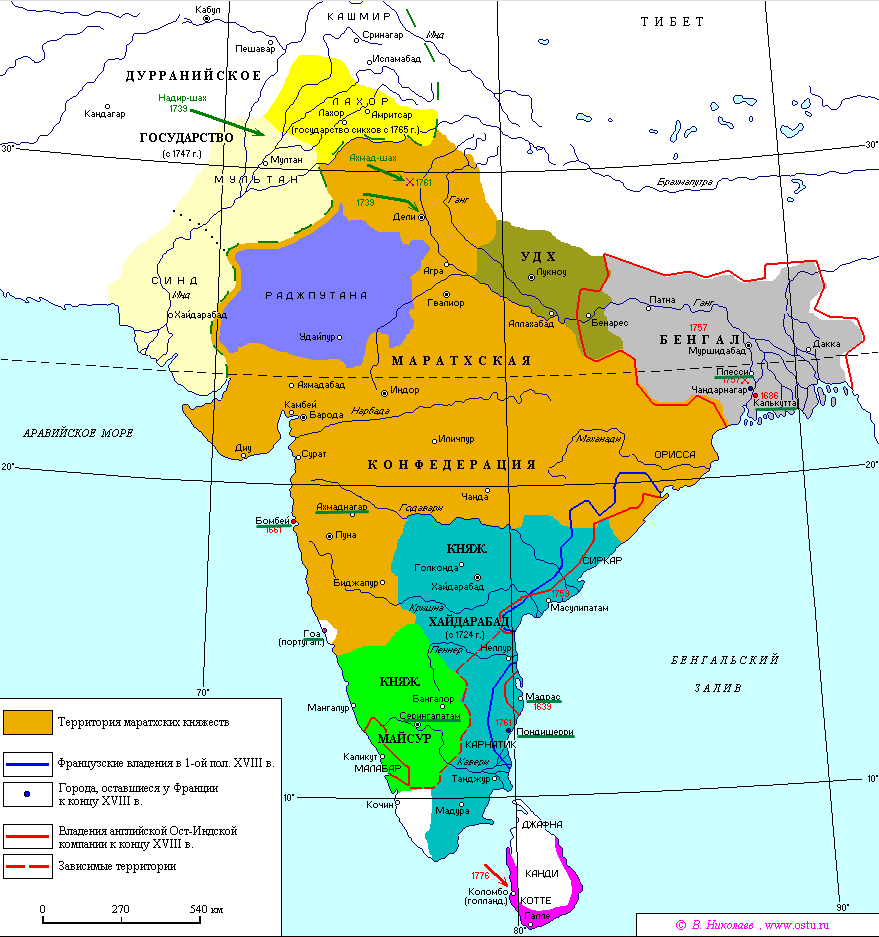
\includegraphics{IndiaMap.png}

\hypertarget{ux43fux440ux43eux43aux43bux430ux43cux430ux446ux438ux44f-ux43cux430ux43bux430ux440ux442ux438ux43aux430}{%
\chapter{Прокламация Малартика}\label{ux43fux440ux43eux43aux43bux430ux43cux430ux446ux438ux44f-ux43cux430ux43bux430ux440ux442ux438ux43aux430}}

\textbf{Свобода. Равенство.\\
Французская Республика, единственная и независимая.\\
Прокламация\\
Анна-Жозефа Ипполита Малартика, главнокомандующего и генерал-губернатора Иль-де-Франса, Реюньона и всех французских ведомств к востоку от мыса Доброй Надежды.}

Граждане,\\
узнав в течение нескольких лет о вашем рвении и вашей приверженности к славе и интересам нашей Республики, мы очень беспокоимся и считаем своим долгом ознакомить вас со всеми предложениями, которые сделал Типу-Султан через двух отправленных к нам послов.

Этот князь написал подробные письма Колониальному собранию, всем генералам, находящимся на службе у этого правительства и направил нам пакет для Исполнительной Директории.

\begin{enumerate}
\def\labelenumi{\arabic{enumi}.}
\item
  Он желает сформировать наступательный и оборонительный союз с французами и предлагает взять на себя все расходы за войска, которые могут быть ему посланы, в течение всей войны в Индии.
\item
  Он обещает предоставить все необходимое для ведения войны, за исключением вина и бренди, которыми он совершенно не обеспечен.
\item
  Он заявляет, что сделает все возможное, чтобы получить помощь, которую мы могли бы ему послать, и что по прибытии войск командиры и офицеры найдут все необходимое для ведения войны, к которой европейцы мало привыкли.
\item
  Одним словом, он ждет того момента, когда французы придут к нему на помощь, чтобы объявить войну англичанам, которых он горячо желает изгнать из Индии.
\end{enumerate}

Поскольку мы не можем сократить количество солдат 107-го и 108-го полков и регулярного караула Пор-Фратерните из-за помощи, предоставляемой нашим союзникам голландцам, мы приглашаем граждан, которые выразят желание стать добровольцами, записаться в своих муниципалитетах на службу под знаменами Типу.

Также этот князь хочет, чтобы ему помогали свободные цветные граждане, поэтому мы приглашаем записаться всех тех, кто желает служить под его флагом.

Мы можем заверить всех граждан, которые решат зарегистрироваться, что Типу предложит им выгодную ставку оплаты, условия которой будут установлены его послами; говорящими от имени своего суверенного правителя, что все французы, которые поступят в ряды его армии, никогда не будут задерживаться, если выразят желание вернуться в родную страну.

\textbf{Пор-Нор-Уэст, 30 января 1798 года\\
(подпись) Малартик}

\end{document}
